\documentclass[11pt]{article}
\usepackage{nth}
\usepackage[hidelinks]{hyperref}
\usepackage{tikz}
\usetikzlibrary{shapes,arrows}
\tikzstyle{line}=[draw]
\usepackage{xcolor}
\usepackage{amsmath}
\usepackage{geometry,blindtext}
\usepackage[edges]{forest}
\usepackage{listings}
\usepackage{color}


\definecolor{dkgreen}{rgb}{0,0.6,0}
\definecolor{gray}{rgb}{0.5,0.5,0.5}
\definecolor{mauve}{rgb}{0.58,0,0.82}



\lstset{frame=tb,
  language=Python,
  aboveskip=3mm,
  belowskip=3mm,
  showstringspaces=false,
  columns=flexible,
  basicstyle={\small\ttfamily},
  numbers=none,
  numberstyle=\tiny\color{gray},
  keywordstyle=\color{blue},
  commentstyle=\color{dkgreen},
  stringstyle=\color{mauve},
  breaklines=true,
  breakatwhitespace=true,
  tabsize=3
}

\def\hiddenparcommand{\par}
\newcommand\otherhiddenparcommand{\par\noindent}
\newcommand\hiddencommacommand{, }
\forestset{%
  declare keylist register={split here ids},
  split here ids={},
  declare keylist register={split here interjects},
  split here interjects={},
  declare keylist={split here auto siblings}{},
  declare toks register=split here toks,
  declare dimen register=tmpdima,
  tmpdima'=0pt,
  declare dimen register=tmpdimb,
  tmpdimb'=0pt,
  declare dimen register=tmpdimc,
  tmpdimc'=0pt,
  to widest/.style={
    tikz+={\path (\forestregister{tempdima}, \forestoption{y}) -- (\forestregister{tempdimb}, \forestoption{y});},
  },
  hide commas/.style={%
    split here toks+={\hiddencommacommand},
    split here toks+={#1},
  },
  split dir tree pre/.style={%
    label={[text=gray, anchor=north, font=\scriptsize]below:{[cont.]}{}},
  },
  split dir tree post/.style={%
    label={[font=\scriptsize, anchor=south, text=gray]above:{[cont.]}{}},
  },
  split dir tree auto post/.style={
    split dir tree post,
    tempkeylistc'={},
    tmpdimb/.option=y,
    for nodewalk={
      while={
        > ORw2+d _+d < On=! & {y}{tmpdimb}{##2-##1} {\textheight-#1} {n'}{1}%
      }{
        next,
        tempkeylistc/.option=name
      }%
    }{},
    % save the list
    split here auto siblings/.register=tempkeylistc,
    tikz+/.process={% this tries to redraw the edges to the following siblings
      OOw2{edge}{id}%
      {%
        \path [##1] (!u.parent anchor |- .north) ++(\forestregister{folder indent},1ex) coordinate (before ##2) |- (.child anchor);
        \edef\tempa{\foresteoption{split here auto siblings}}
        \foreach \i in \tempa \path [##1] (before ##2) |- ({forest cs:\i.child anchor});
      }%
    },
  },
  split dir tree/.code={%
    \forestset{%
      draw tree stage/.style={
        for root'={
          tempdima/.min={%
            >OOw2+d{x}{min x}{####1+####2}%
          }{tree},
          tempdimb/.max={%
            >OOw2+d{x}{max x}{####1+####2}%
          }{tree},
          for tree={%
            to widest,
          },
        },
        tempcountb'=-1,
        do until={%
          strequal((split_here_ids),"")
        }{%
          tempkeylistb'={},
          tempkeylista'={},
          split register={split here ids}{,}{tempcounta,tempkeylistb+},
          split register={split here interjects}{,}{temptoksa,tempkeylista+},
          split here ids'/.register=tempkeylistb,
          split here interjects'/.register=tempkeylista,
        % Sašo Živanović: http://chat.stackexchange.com/transcript/message/28484520#28484520
         for nodewalk={%
           draw tree processing order/.style={%
             filter={tree}{> ORw+n< OR> & {id}{tempcounta}{########1+1}{id}{tempcountb}}%
           }%
         }{},
          for root'={draw tree},
          TeX/.process={Rw{temptoksa}{\otherhiddenparcommand ####1\hiddenparcommand}},
          tempcountb'/.register=tempcounta,
        },
        for nodewalk={%
          draw tree processing order/.style={%
            filter={tree}{>OR>{id}{tempcountb}}%
          }%
        }{},
        for root'={draw tree},
      },
    }%
  },
  split dir here auto/.style n args=2{%
    split dir tree pre,
    !next node.split dir tree auto post=#2,
    split here ids+/.option=id,
%     !next node.split resume here ids+/.option=id,
    split={#1}{,}{split here toks,hide commas},
    split here interjects/.register=split here toks,
  },
  split dir tree auto/.style={%
    split dir tree,
    before drawing tree={%
      tempdima/.max={y}{tree},
      tempdimc/.register=tempdima,
      tempdimd/.min={y}{tree},
      tempdima-/.register=tempdimd,
      tempdimb'=\textheight,
      tmpdima'=10ex,
      tmpdimc'=\pagetotal,
      while={%
        >RR>{tempdima}{tempdimb}%
      }{%
        for nodewalk={%
          root',
          until={%
            > ROw2+d RRw2+d > {tempdimc}{y}{##1-##2} {tmpdima}{tmpdimc}{\textheight-##2-##1}%
          }{next node},
          previous node,
          split dir here auto/.process={R_w2{tmpdima}{continued}{{##2}{##1}}},
          next node,
          tempdima/.option=y,
          tempdimc/.register=tempdima,
          tempdima-/.register=tempdimd,
          tmpdima'=15ex,
          tmpdimc'=0pt
        }{},
      },
    },
  },
}

\begin{document}
\title{OpenSBLI user manual and developer guide}
\author{David J. Lusher, Satya P. Jammy, Neil D. Sandham}
% \date
\maketitle


\section*{OpenSBLI user manual, major revision history:}
\begin{itemize}
  \item{OpenSBLI Version 3.0 release updates, multi-block: DJL - October 2024.}
  \item{Update for CPC Version 2.0 paper publication: DJL - June 2021.}
  \item{Added non-linear WENO filter methods: DJL - September 2020.}
  \item{Added Python 3 compatibility: DJL - May 2020.}
	\item{Initial version: DJL - March 2020.}
\end{itemize}

\noindent \underline{The latest references for OpenSBLI are the following:}

\begin{itemize}
  
\item D.J. Lusher, A. Sansica, N.D. Sandham, J. Meng, B. Siklósi, A. Hashimoto. OpenSBLI v3.0: High-Fidelity Multi-Block Transonic Aerofoil CFD Simulations using Domain Specific Languages on GPUs. \textbf{Computer Physics Communications, 109406 (2024)}.

\item D.J. Lusher, S.P. Jammy, N.D. Sandham. OpenSBLI: Automated code-generation for heterogeneous computing architectures applied to compressible fluid dynamics on structured grids. \textbf{Computer Physics Communications Vol. 267, 108063 (2021)}.


\end{itemize}

\section*{Introduction}

\subsection*{Quick start: General work flow}
Below are the five main steps that must be performed to generate a code in OpenSBLI and run it within OPS. Please see section \ref{sec:installation_guide} for detailed instructions on how to install OpenSBLI, OPS, and run a simulation. 

\begin{enumerate}
\item{Run \verb|python problem_file.py| for one of the problem files located in the apps folder in OpenSBLI to generate a C code.}
\item{Copy the C code \verb|(*.cpp, *.h)| files to the machine where you have OPS installed to run the simulations.}
\item{Use the OPS source-to-source translator on the \verb|opensbli.cpp| file to generate parallel versions of the code (OpenMP, OpenACC, MPI, CUDA, OpenCL, ...)}
\item{Copy a Makefile into the working directory and compile the code: \verb|make opensbli_mpi|.}
\item{Run the executable: \verb|mpirun -np 4 ./opensbli_mpi|.}
\end{enumerate}

\noindent\textbf{Important note:} The purpose of OpenSBLI is to generate a complete CFD simulation code in the C language from a set of user-defined equations and options. The execution of the simulation code to obtain results is performed with the OPS library. The OPS library must be built on whichever machine you wish to run the simulation on. Codes can be generated locally on a laptop in OpenSBLI and then copied onto a high-performance computing cluster to run with OPS. In many cases once a C code has been generated in OpenSBLI, changes can be made to the C code directly without needing to generate another code through the OpenSBLI Python interface.

\newpage
\tableofcontents

\newpage
\section{Installation guide}\label{sec:installation_guide}
OpenSBLI requires a Python 3 installation for code generation and the Oxford Parallel Structured software (OPS) library to build executables. The guide is for Linux platforms only, it hasn't been tested on OSX/Windows. Section 1 outlines the libraries that must be installed to use OpenSBLI + OPS, section 2 explains the build process of OPS, section 3 covers how to generate a code within OpenSBLI and section 4 gives the steps to compile and run the code. Section 5 has some additional information that may be applicable if running on an HPC cluster.


The installation of libraries will depend on whether you are using a local machine or an HPC cluster. If you are intending to use OpenSBLI on an HPC cluster you will need to load suitable system modules and point OPS to them via the environment variables outlined in section \ref{sec:OPS}. MPI and HDF5 libraries must have been compiled with the same compiler or you will face errors during compilation of OPS executables. If you are not sure where the  modules are located, please contact your system administrator. \textbf{Important note: SymPy version 1.1 is required, newer versions are currently not supported.} The requirements are:
\subsection*{OpenSBLI requirements (Python 3)}
\begin{verbatim}
Python versions 3 <= 3.7*
SymPy version 1.1 : Symbolic Python libary used by OpenSBLI
Matplotlib : Python plotting library
h5py : Python library to read in HDF5 output files for plotting
NumPy : Numerical Python library used in some plot scripts
SciPy: Scientific Python library used in some OpenSBLI classes
\end{verbatim}
\subsection*{OPS requirements}
\begin{verbatim}
git : Version control software used to clone the repository
A C compiler : (gcc, icc, Cray, ..)
An MPI distribution : (OpenMPI, MPICH, Intel MPI, ..)
HDF5 libraries : Used for I/O within OPS
CUDA/OpenCL libraries : Required only if you intend to run on GPUs
\end{verbatim}
\textbf{Note:} Codes can be generated with OpenSBLI on a local machine (laptop) and copied onto another machine to be translated, compiled and run with OPS. While you can install both OpenSBLI and OPS on an HPC cluster, it is not necessary to have both on the same machine. OPS however must be installed (and built) on the machine you wish to run simulations on.


\noindent \textbf{Python 3.8*:} this version of Python is supported with the following patch to SymPy (modify \verb|<base_python_dir>| as appropriate for your system):

\begin{lstlisting}
sed -i -e "s/value=ast.Name/value=ast.NameConstant/g" <base_python_dir>sympy/parsing/sympy_parser.py
sed -i -e "s/id='False'/value=False/g" <base_python_dir>/sympy/parsing/sympy_parser.py
\end{lstlisting}

\subsection{Installation of libraries on an Ubuntu local machine}
\textbf{**Ignore this section if installing OpenSBLI on an HPC cluster**}\\
This section was tested on a clean Ubuntu 18.04 LTS installation, similar packages can be found for other Linux distributions. Python packages are installed with pip, if pip is not already present on your system it can be installed with e.g. \verb|sudo apt-get install python-pip|, on Ubuntu/Debian based systems. Alternatively, software distributions like Anaconda can be used to install the Python libraries. The guide is for installation on a local machine with the GNU C compiler (gcc) and OpenMPI.

\begin{enumerate}
\item{Install OpenMPI and HDF5 libraries, git and pip/tk
\begin{verbatim}
sudo apt-get install python-pip python-tk
sudo apt-get install libhdf5-openmpi-dev
sudo apt-get install git
\end{verbatim}}
\item{Install the required Python packages for this user. Note that SymPy 1.1 is required, more recent versions will cause issues:}
\begin{verbatim}
pip install --user scipy numpy h5py matplotlib
pip install --user sympy==1.1
\end{verbatim}

\end{enumerate}


\subsection{OPS installation}\label{sec:OPS}
In this section the installation of the OPS library is explained. \textbf{The paths that you put in step 2 will change depending on whether you are on a local machine or an HPC cluster.}
\begin{enumerate}
\item{Clone the OPS library:\\ \verb|git clone https://github.com/OP-DSL/OPS.git|}
\item{Export OPS environment variables:\\ Edit your \verb|~/.bashrc| to include the lines:}
\subsection*{Local Ubuntu machine:}
\begin{verbatim}
export OPS_INSTALL_PATH=/home/<username>/OPS/ops/
export OPS_COMPILER=gnu
export OPS_TRANSLATOR=/home/<username>/OPS/ops_translator/c/
export MPI_INSTALL_PATH=/usr/
export HDF5_INSTALL_PATH=/usr/lib/x86_64-linux-gnu/hdf5/openmpi/
export CUDA_INSTALL_PATH=/path/to/cuda-install/
export USE_HDF5=1
\end{verbatim}

\subsection*{HPC cluster: (fill these in)}
\begin{verbatim}
export OPS_INSTALL_PATH=/home/<username>/OPS/ops/
export OPS_COMPILER=gnu/cray/intel (pick one)
export OPS_TRANSLATOR=/home/<username>/OPS/ops_translator/c/
export MPI_INSTALL_PATH=/path/to/mpi-install/
export HDF5_INSTALL_PATH=/path/to/hdf5-install/
export CUDA_INSTALL_PATH=/path/to/cuda-install/
export USE_HDF5=1
\end{verbatim}
To make these changes active in the current shell type: \verb|source ~/.bashrc|
\item{Build the OPS libraries:}
\begin{verbatim}
Change directory to ~/OPS/ops/c/
make seq mpi hdf5_seq hdf5_mpi
\end{verbatim}
If you are using CUDA/OpenCL for GPUs you will also have to build:
\begin{verbatim}
make cuda mpi_cuda opencl mpi_opencl
\end{verbatim}
You may see some warnings that can be ignored, the ./lib/ folder should now contain some OPS libraries. If you encounter errors at this point it will be due to improper configuration of the modules/environment variables.
\end{enumerate}

\subsection{OpenSBLI installation and code generation}
\begin{enumerate}
\item{Clone the latest OpenSBLI with your username and switch branch:}
\begin{verbatim}
git clone https://github.com/opensbli/opensbli.git
\end{verbatim}

\item{Export the OpenSBLI folder to your PYTHONPATH in \verb|~/.bashrc|:}
\begin{verbatim}
export PYTHONPATH=$PYTHONPATH:/home/<username>/opensbli/
source ~/.bashrc
\end{verbatim}

\item{Generate a code in OpenSBLI (e.g. Taylor-Green vortex):}
\begin{verbatim}
cd apps/taylor_green_vortex/
python taylor_green_vortex.py
\end{verbatim}
You should now have eight new files:\\ \verb|opensbli.cpp, opensbliblock00_kernels.h, defdec_data_set.h, bc_exchanges.h|\\
\verb|stencils.h, io.h, reductions.h, constants.h|, and some LaTeX files.
\end{enumerate}
At this point the files may be copied onto another machine (if desired) where you have OPS installed. The OPS translation and compilation steps are described in the next section.


\subsection{Compiling and running the code}\label{sec:compiling_code}
\begin{enumerate}
\item{Translate the code using OPS to generate parallel versions:}
\begin{verbatim}
python $OPS_TRANSLATOR/ops.py opensbli.cpp
\end{verbatim}
You should now have folders for CUDA, MPI and so on, plus an \verb|opensbli_ops.cpp| file. You need to apply the translation step each time you make changes to the opensbli.cpp code generated by OpenSBLI. Ignore the clang-format warning, this is just an optional code indentation formatter and has no effect on the simulation.

\item{Copy a Makefile into the directory and build the executable for the desired architecture (MPI, CUDA, OpenMP etc):}
\begin{verbatim}
cp ../Makefile ./
make opensbli_mpi
\end{verbatim}

\item{Run the executable for number of processes 'np':}
\begin{verbatim}
mpirun -np 4 ./opensbli_mpi
\end{verbatim}
The simulation will now run, when finished the output data is written to an \verb|opensbli_output.h5| HDF5 file for post-processing. If you wish to run the simulation again remove the HDF5 file from the directory before repeating the above steps as existing files won't be overwritten.

\end{enumerate}

\subsection{Things to note for HPC clusters:}
\begin{enumerate}
\item{For different compilers the \verb|OPS_COMPILER| variable set in section \ref{sec:OPS} must be changed and you may need to modify some of the Makefiles. The easiest way is usually to export cc and CC to where your compiler is located, but you may need to explicitly edit the Makefiles to use icc/icpc for example. In the current OPS, the Makefiles are all located in /OPS/makefiles/}

\item{If there is no suitable HDF5 available on the system you will have to build it yourself:}
\begin{verbatim}
Obtain the source: https://support.hdfgroup.org/HDF5/release/obtainsrc.html
Extract the file, change to the directory and configure the build.
For building parallel HDF5:
./configure --enable-parallel cc=/path/to/mpicc CC=/path/to/mpicc
make
make install
\end{verbatim} 

\item{Depending on the machine you may need to add your HDF5/CUDA library locations to your \verb|LD_LIBRARY_PATH| environment variable.}

\item{Job submission scripts will often need module load commands in them as the compute nodes are separate to login nodes. In addition \verb|LD_LIBRARY_PATH| may need to be exported in the submission script with the HDF5/CUDA library locations.}

\item{If using gcc you may need to add:}
\begin{verbatim}
-fpermissive to CCFLAGS/CXXFLAGS in OPS/makefiles/Makefile.gnu
\end{verbatim}

\end{enumerate}

\newpage
\section{List of source code files}
\subsection{Directory structure}
The directory tree below shows the structure of the OpenSBLI source code files. Folders are highlighted in blue and files in black.

\begin{forest}
  for tree={
    folder,
    grow'=0,
    fit=band,
  },
  split dir tree auto,
      [\textcolor{blue}{OpenSBLI base directory}
      [\textcolor{blue}{apps}
      [aerofoils]
      [channel\_flow]
      [compressible\_taylor\_green\_vortex]
      [cylinder]
      [euler\_wave]
      [euler\_wave\_curvilinear]
      [flat\_plate\_transition]
      [inviscid\_shock\_reflection]
      [katzer\_SBLI]
      [kelvin\_helmholtz]
      [Lax\_shock\_tube]
      [LeBlanc]
      [mixing\_layer]
      [not-finished]
      [performance\_benchmark]
      [shu\_osher]
      [Sod\_shock\_tube]
      [taylor\_green\_vortex]
      [transitional\_SBLI]
      [turbulent\_counter\_flow]
      [viscous\_shock\_tube]
      [vortex\_core]
      [wave]
      ]
      [\textcolor{blue}{docs}
      ]
      [\textcolor{blue}{opensbli}
        [\textcolor{blue}{code\_generation} [\textcolor{blue}{algorithm} [algorithm.py]]
        ] [latex.py] [opsc.py]
        [\textcolor{blue}{core} [bcs.py] [block.py] [datatypes.py] [grid.py]
        [io.py] [kernel.py] [opensblifunctions.py] [opensbliobjects.py] [parsing.py]
        [\textcolor{blue}{diagnostics} [residual\_monitor.py] [simulation\_monitor.py]
        ]
        ]
        [\textcolor{blue}{equation\_types} [metric.py] [opensbliequations.py]
        ]
        [\textcolor{blue}{filters} [DRP\_filter.py] [SFD.py] [TVD\_filter.py] [WENO\_filter.py] [binomial\_filter.py]
        ]
        [\textcolor{blue}{initialisation} [gridbasedinit.py]
        ]
        [\textcolor{blue}{multiblock} [algorithm.py] [blockcollection.py]
        ]
        [\textcolor{blue}{optimisations} [StoreSome.py]
        ]
      	[\textcolor{blue}{physical\_models} [euler\_eigensystem.py] [ns\_physics.py] [split\_forms.py]
      	]
      	[\textcolor{blue}{post\_process} [airfoil.py] [plot\_functions.py] [post\_process\_eq.py] [removehalos.py] [tecplot2D.py]
      	]
      	[\textcolor{blue}{schemes} [\textcolor{blue}{spatial}
      	[averaging.py] [scheme.py] [shock\_capturing.py] [shock\_sensors.py] [TVD.py] [teno.py] [weno.py] ] [\textcolor{blue}{temporal}
      	[rk\_LS.py] [rk\_sbli.py]]
      	]
      	[\textcolor{blue}{utilities} [helperfunctions.py] [katzer\_init.py] [numerical\_functions.py] [oblique\_shock.py] [user\_defined\_kernels.py]
      	]
      ]
    ]
\end{forest}

\subsection{Description of the source code files}
This is a brief description of each of the source code files.
\begin{enumerate}
	\item{\textbf{algorithm.py:} Placement and ordering of the different solution components in the output code. Defines the iteration and sub-stage loops and their respective components.}
	\item{\textbf{averaging.py:} Simple (mean) and Roe averaging routines for the characteristic decomposition. Used for the shock-capturing schemes.}
	\item{\textbf{bcs.py:} All of the boundary conditions defined in OpenSBLI. Also contains the one-sided boundary derivative schemes.}
	\item{\textbf{block.py:} The simulation block contains grid information and links all of the main OpenSBLI components together.}
	\item{\textbf{datatypes.py:} Floating point precision definitions.}
	\item{\textbf{euler\_eigensystem.py:} Definitions of the transformation matrices used in the characteristic decomposition of the Euler equations. Used for improving the robustness of the shock-capturing schemes.}
	\item{\textbf{grid.py:} Defines the parameters related to the grid (sizes, ranges) and the declaration of global work arrays.}
	\item{\textbf{gridbasedinit.py:} The class used to initialise the solution at $t=0$. Equations given to the initialisation class are calculated once at the start of the simulation.}
	\item{\textbf{helperfunctions.py:} Miscellaneous functions frequently used throughout the internal structure of OpenSBLI. It also contains routines for adding the problem-specific HDF5 metadata required by OPS for reading/writing files.}	
	\item{\textbf{hybrid.py:} Routines for hybrid central-WENO schemes via a shock sensor.}
	\item{\textbf{io.py:} The main input/output class controlling reading and writing of simulation data within OpenSBLI.}
	\item{\textbf{katzer\_init.py:} Numerical similarity solution of the compressible boundary-layer equations. Creates laminar boundary-layer profiles for wall-bounded domain initialisation.}	
	\item{\textbf{kernel.py:} The main class for OpenSBLI kernels which perform a computation for a given kernel range in parallel.}
	\item{\textbf{latex.py:} Functionality to convert symbolic equations in OpenSBLI to TeX format. The output can be compiled with pdflatex to produce a pdf file.}
	\item{\textbf{metric.py:} Classes to perform the metric transformation to generalised curvilinear coordinates.}
  \item{\textbf{multiblock/algorithm.py:} Implementation of the algorithm class for multi-block problems.}
  \item{\textbf{multiblock/blockcollection.py:} Helper functions for multi-block implementation.}
	\item{\textbf{numerical\_functions.py:} Numerical spline interpolation routines used for the similarity solution. These functions are for creating initial profiles in Python and are not part of the output simulation.}	
	\item{\textbf{ns\_physics.py:} A physics object containing frequently used definitions related to the compressible Navier-Stokes equations.}
	\item{\textbf{oblique\_shock.py:} Oblique shock jump relation calculator.}		
	\item{\textbf{opensbliequations.py:} The main file for defining equations in OpenSBLI. Contains the routines for the SimulationEquations and ConstituentRelation classes.}
	\item{\textbf{opensblifunctions.py:} Definitions of common derivative objects (Central, WENO, TENO) and the EinsteinStructure for indexing symbolic quantities in OpenSBLI.}
	\item{\textbf{opensbliobjects.py:} Definitions of various symbolic objects within OpenSBLI that can be used to build up symbolic equations.}
	\item{\textbf{opsc.py:} This controls the conversion of symbolic objects to C code compliant with the OPS domain-specific language.}	
	\item{\textbf{parsing.py:} Routines to parse equations written as Python strings into equations comprised of symbolic objects.}	
	\item{\textbf{post\_process\_eq.py:} A class to create a post processing OPS code.}
	\item{\textbf{removehalos.py:} Functionality to strip halo points from OpenSBLI output HDF5 files.}	
	\item{\textbf{rk\_LS.py:} Low-storage explicit Runge-Kutta schemes in the two-register Williamson formulation. Contains schemes for \nth{3}, \nth{4} order and \nth{3} order with strong-stability-preservation (SSP).}
	\item{\textbf{rk\_sbli.py:} Low-storage explicit \nth{3} order Runge-Kutta scheme in the form used in the old SBLI Fortran code.}	
	\item{\textbf{scheme.py:} Contains the central differencing scheme and coefficient generator for the finite difference stencils.}
  \item{\textbf{SFD.py:} Selective-Frequency-Damping low-pass temporal filter for generating steady solutions.}
	\item{\textbf{shock\_capturing.py:} All of the common functionality for the characteristic decomposition shared between the various WENO/TENO shock-capturing schemes.}
	\item{\textbf{shock\_sensors.py:} The modified Ducros shock sensor.}
  \item{\textbf{simulation\_monitor.py:} Point-based probes to log histories at individual grid points within the flow-field.}
  \item{\textbf{split\_forms.py:} Quadratic- and cubic-split forms of the convective terms of the Navier-Stokes equations.}
  \item{\textbf{StoreSome.py:} Optimisations for reduced work array usage for central-based schemes.}
	\item{\textbf{teno.py:} Routines for the Targeted Essentially Non-Oscillatory (TENO) shock-capturing schemes.}
    \item{\textbf{TVD\_filter.py:} Application of a TVD scheme once at the end of each full Runge-Kutta time-step. To be used in conjunction with a base central scheme.}
	\item{\textbf{user\_defined\_kernels.py:} Functionality to generate one-off OpenSBLI kernels. Useful for non-standard processing or filtering operations that the user may want to add to their simulation.}	
	\item{\textbf{weno.py:} Routines for the Weighted Essentially Non-Oscillatory (WENO) shock-capturing schemes. Including the WENO-JS and WENO-Z formulations.}
  \item{\textbf{WENO\_filter.py:} Application of the WENO schemes once at the end of each full Runge-Kutta time-step. To be used in conjunction with a base central scheme.}
\end{enumerate}

\newpage
\section{Example problem script for creating a simulation code}
In this section the components of an example problem script are shown for guidance of how to set up a problem in OpenSBLI. The selected problem is the laminar two-dimensional shock-wave/boundary-layer interaction Katzer case (Katzer (1989), JFM 206, pp. 477-496).

\subsection{Defining the governing equations}
\begin{lstlisting}
#!/usr/bin/env python
from opensbli import *
import copy
from opensbli.utilities.katzer_init import Initialise_Katzer
from opensbli.utilities.helperfunctions import substitute_simulation_parameters
\end{lstlisting}
The first step imports all of the classes from the OpenSBLI source code and some individual components used for the Katzer SBLI case.

\begin{lstlisting}
ndim = 2
sc1 = "**{\'scheme\':\'Teno\'}"
# Define the compresible Navier-Stokes equations in Einstein notation.
mass = "Eq(Der(rho,t), - Conservative(rhou_j,x_j,%s))" % sc1
momentum = "Eq(Der(rhou_i,t) , -Conservative(rhou_i*u_j + KD(_i,_j)*p,x_j , %s) + Der(tau_i_j,x_j) )" % sc1
energy = "Eq(Der(rhoE,t), - Conservative((p+rhoE)*u_j,x_j, %s) - Der(q_j,x_j) + Der(u_i*tau_i_j ,x_j) )" % sc1
stress_tensor = "Eq(tau_i_j, (mu/Re)*(Der(u_i,x_j)+ Der(u_j,x_i) - (2/3)* KD(_i,_j)* Der(u_k,x_k)))"
heat_flux = "Eq(q_j, (-mu/((gama-1)*Minf*Minf*Pr*Re))*Der(T,x_j))"
# Substitutions
substitutions = [stress_tensor, heat_flux]
constants = ["Re", "Pr", "gama", "Minf", "SuthT", "RefT"]
\end{lstlisting}
The user selects the number of dimensions and specifies the conservative derivatives should be discretized by a Targeted Essentially Non-Oscillatory (TENO) scheme by passing the scheme name as an argument into the equation strings. The continuity, momentum and energy equations are defined from the compressible Navier-Stokes equations. To improve readability the stress tensor $\tau_{i,j}$ and heat flux terms $q_j$ are defined separately to be substituted into the momentum and energy equations. The equations are defined as strings to be parsed into symbolic quantities by OpenSBLI. The SymPy \verb|Eq| class is used to define the equations, with the temporal and spatial derivatives separated into the left and right hand side of the equation respectively. The final line defines a list of constant quantities required by the simulation.

\subsection{Defining constituent relations}
\begin{lstlisting}
# Define coordinate direction symbol (x) this will be x_i, x_j, x_k
coordinate_symbol = "x"
# Formulas for the variables used in the equations
velocity = "Eq(u_i, rhou_i/rho)"
pressure = "Eq(p, (gama-1)*(rhoE - rho*(1/2)*(KD(_i,_j)*u_i*u_j)))"
speed_of_sound = "Eq(a, (gama*p/rho)**0.5)"
temperature = "Eq(T, p*gama*Minf*Minf/(rho))"
viscosity = "Eq(mu, (T**(1.5)*(1.0+SuthT/RefT)/(T+SuthT/RefT)))"
\end{lstlisting}
A symbolic letter is selected to perform the spatial expansion over the indices in the governing equations. The next five lines are definitions to be used in the \verb|ConstituentRelations| class. These formulae tell OpenSBLI how to evaluate quantities present in the governing equations that have not yet been defined. In this example the primitive variables of pressure, temperature, and directional velocity components are defined as functions of the conservative variables in the governing equations. As this problem is set up to use shock capturing schemes the speed of sound $a$ must also be defined. For this supersonic test case the viscosity $\mu(T)$ is a function of temperature using Sutherland's law. If constant viscosity was required instead this equation could be omitted and mu could be defined as a constant as above.

\subsection{Parsing and expanding the equations into symbolic expressions}
\begin{lstlisting}
# Instatiate equation classes
eq = EinsteinEquation()
base_eqns = [mass, momentum, energy]
constituent_eqns = [velocity, pressure, speed_of_sound, temperature, viscosity]
# Expand the base equations
for i, base in enumerate(base_eqns):
    base_eqns[i] = eq.expand(base, ndim, coordinate_symbol, substitutions, constants)
# Expand the constituent relations
for i, CR in enumerate(constituent_eqns):
    constituent_eqns[i] = eq.expand(CR, ndim, coordinate_symbol, substitutions, constants)
\end{lstlisting}

Having defined the governing equations and constituent relations, the next task is to use OpenSBLI to parse and expand these equations over the number of specified dimensions. The \verb|EinsteinEquation| class is instantiated to perform expansions, and the equations defined previously are added to lists so they can be expanded iteratively in a Python loop. The expansion routine takes the input equation, number of dimensions, coordinate symbol and any substitutions and constants defined. The output is a symbolic version of each of the governing equations. The same approach is used for the five constituent relations defined by the user.

\subsection{Creating a simulation block and generating coordinate transformations}\label{sec:applying_transformation}
\begin{lstlisting}
block = SimulationBlock(ndim, block_number=0)
# Create metrics before the scheme selection
metriceq = MetricsEquation()
metriceq.generate_transformations(ndim, coordinate_symbol, [(False, False), (True, False)], 2)
\end{lstlisting}
In this step the simulation block is created based on the number of dimensions. For this wall bounded flow we apply grid stretching normal to the wall to improve the grid resolution in the boundary layer. To do this the \verb|MetricsEquation| class is created and then transformation matrices are generated by specifying which directions of the problem require a coordinate transformation. The tuples \verb|(False, False)| refer to whether grid stretching and curvilinear coordinates are required for a given direction. In this example curvilinear coordinates are turned off and only grid stretching is requested in the second spatial direction.

\subsection{Transformation of the simulation equations}
\begin{lstlisting}
# Create SimulationEquations and Constituent relations, add the expanded equations
simulation_eq = SimulationEquations()
constituent = ConstituentRelations()
for eqn in base_eqns:
    simulation_eq.add_equations(eqn)
for eqn in constituent_eqns:
    constituent.add_equations(eqn)
# Grid is stretched normal to the wall
simulation_eq.apply_metrics(metriceq)
\end{lstlisting}
To store the governing equations a \verb|SimulationEquations| class is instantiated and the previously expanded equations are added to it with the \verb|add_equation| routine. The same procedure is applied to store the expanded constituent relation equations. In the final line the previously created metric class is used to transform the derivatives in the simulation equations.

\subsection{Numerical scheme selection}
\begin{lstlisting}
# Adaptive TENO with modified Ducros sensor
SS = ShockSensor()
shock_sensor, sensor_array = SS.ducros_equations(block, coordinate_symbol, metriceq)
# Add shock Ducros sensor to constituent relations
constituent.add_equations(shock_sensor)
store_sensor = True
teno_order = 5
Avg = RoeAverage([0, 1])
LLF = LLFTeno(teno_order, formulation='adaptive', averaging=Avg, sensor=sensor_array, store_sensor=True)
schemes = {}
schemes[LLF.name] = LLF
\end{lstlisting}

At this point we specify the numerical schemes to be used to discretize the governing equations. For this example we are using the adaptive TENO scheme which requires a shock sensor to be provided. The shock sensor class is instantiated and the Ducros sensor is selected. As the Ducros sensor contains derivative quantities the metric class must be provided to perform the necessary coordinate transformations. The equation to evaluate the shock sensor is then added to the constituent relations to be computed at the start of each sub-stage in the time loop. A \nth{5} order scheme is selected with the Roe averaging option for the characteristic decomposition. The \verb|LLFTeno| class is selected to perform local Lax-Friedrichs flux splitting with a TENO scheme. An empty dictionary is created to hold the schemes, to which the LLF class is added. Note that when using the TENO schemes a value of $\epsilon = 1\times 10^{-15}$ should be specified in the simulation constants list.

\begin{lstlisting}
cent = Central(4)
schemes[cent.name] = cent
rk = RungeKuttaLS(3, formulation='SSP')
schemes[rk.name] = rk
block.set_discretisation_schemes(schemes)
\end{lstlisting}
Having selected the scheme to discretize the convective terms NS equations, we must now select a scheme for the viscous and heat-flux terms. This is done by creating a Central differencing class of order 4 and adding it to the scheme dictionary. A \nth{3} order low-storage SSP Runge-Kutta scheme is then selected to perform the explicit time integration. The final step is to set the chosen schemes on the simulation block for later use.

\subsection{Creating boundary conditions}
For a 2D problem we have to specify four boundary conditions. The convention we use for each boundary condition is to apply the coordinate direction and then 0 or 1 for the two possible sides in that direction. For this 2D shock-wave/boundary-layer interaction the possible combinations are $[0,0]$ and $[0,1]$ for the inlet and outlet in the $x_0$ direction, plus $[1,0]$ and $[1,1]$ for the no-slip wall and upper shock jump conditions in $x_1$. 

\begin{lstlisting}
boundaries = [[0, 0] for t in range(ndim)]
# Left pressure extrapolation at x= 0, inlet conditions
direction = 0
side = 0
boundaries[direction][side] = InletPressureExtrapolateBC(direction, side)
# Right extrapolation at outlet
direction = 0
side = 1
boundaries[direction][side] = ExtrapolationBC(direction, side, order=0)
\end{lstlisting}
The first step creates a list of lists to hold the four boundary conditions. The inlet $[0,0]$ is then selected as a pressure extrapolation boundary condition that only has the direction and side as input arguments. A simple zero order spatial extrapolation condition is selected for the outlet boundary.

\begin{lstlisting}
local_dict = {"block": block, "GridVariable": GridVariable, "DataObject": DataObject}
# Bottom no-slip isothermal wall
direction = 1
side = 0
wall_const = ["Minf", "Twall"]
for con in wall_const:
    local_dict[con] = ConstantObject(con)
# Isothermal wall condition
rhoE_wall = parse_expr("Eq(DataObject(rhoE), DataObject(rho)*Twall/(gama*(gama-1.0)*Minf**2.0))", local_dict=local_dict)
wall_eqns = [rhoE_wall]
boundaries[direction][side] = IsothermalWallBC(direction, 0, wall_eqns)
\end{lstlisting}
At the bottom of the domain an isothermal no-slip wall is selected. A local dictionary with common OpenSBLI objects is created as the isothermal wall requires an equation for how the user wants to evaluate energy for this boundary condition. Two constants relating to the freestream Mach number and a constant wall temperature are created using the \verb|ConstantObject| class. In this example the parser is used directly to parse the energy equation that has been defined by the user. The last step creates the isothermal wall boundary condition and passes the energy equation as the final function argument.


\begin{lstlisting}
# Top dirichlet shock generator condition
direction = 1
side = 1
x_loc = parse_expr("Eq(GridVariable(x0), block.deltas[0]*block.grid_indexes[0])", local_dict=local_dict)
rho = parse_expr("Eq(DataObject(rho), Piecewise((1.129734572, (x0)>40.0), (1.00000596004, True)))", local_dict=local_dict)
rhou0 = parse_expr("Eq(DataObject(rhou0), Piecewise((1.0921171, (x0)>40.0), (1.00000268202, True)))", local_dict=local_dict)
rhou1 = parse_expr("Eq(DataObject(rhou1), Piecewise((-0.058866065, (x0)>40.0), (0.00565001630205, True)))", local_dict=local_dict)
rhoE = parse_expr("Eq(DataObject(rhoE), Piecewise((1.0590824, (x0)>40.0), (0.94644428042, True)))", local_dict=local_dict)

upper_eqns = [x_loc, rho, rhou0, rhou1, rhoE]
boundaries[direction][side] = DirichletBC(direction, side, upper_eqns)
block.set_block_boundaries(boundaries)
\end{lstlisting}
The fourth boundary condition is a Dirichlet condition to impose flow conditions before and after the oblique shock-wave. As this condition has a dependence on the $x_0$ coordinate we create a local equation to evaluate the current $x_0$ position during the simulation. The next four equations give the pre and post shock values for a $\theta=3.08^{\circ}$ oblique shock at Mach 2. The SymPy class \verb|Piecewise| is used to create an if-else condition dependent on the local $x_0$ coordinate value. 

It is important to note here that the $x_0$ value is stored as a temporary \verb|GridVariable| before being used to set the conservative arrays of type \verb|DataObject| which are stored globally throughout the simulation. The parsed equations are added to a list and then passed as an argument to the \verb|DirichletBC| class. Having selected all four boundary conditions for the problem, they are set on the block in the last line. 



\subsection{Initialisation of the domain and grid}
At this stage we need to select how the domain should be initialised and details of the grid equations. In OpenSBLI a grid can either be read in from a pre-computed HDF5 file or evaluated at runtime in the initialisation kernel. For this example the grid is specified as equations and added to the initialisation. 
\begin{lstlisting}
# Reynolds number, Mach number and free-stream temperature for the initial profile
Re, xMach, Tinf = 950.0, 2.0, 288.0
polynomial_directions = [(False, DataObject('x0')), (True, DataObject('x1'))]
n_poly_coefficients = 50
grid_const = ["Lx1", "by"]
for con in grid_const:
    local_dict[con] = ConstantObject(con)
gridx0 = parse_expr("Eq(DataObject(x0), block.deltas[0]*block.grid_indexes[0])", local_dict=local_dict)
gridx1 = parse_expr("Eq(DataObject(x1), Lx1*sinh(by*block.deltas[1]*block.grid_indexes[1]/Lx1)/sinh(by))", local_dict=local_dict)
coordinate_evaluation = [gridx0, gridx1]
initial = Initialise_Katzer(polynomial_directions, n_poly_coefficients,  Re, xMach, Tinf, coordinate_evaluation)
\end{lstlisting}
For this SBLI case we initialise the domain with a similarity solution laminar boundary layer. The inputs for this routine are the Reynolds number based on inlet displacement thickness, the freestream Mach number and the reference temperature. The initialisation numerically solves the compressible boundary-layer equations in Python to get numerical profiles for $u$ velocity and temperature. A high-order polynomial curve is then fitted to the profiles to create an algebraic expression in $x_1$ that can be evaluated at runtime throughout the domain.

In this case there is only one boundary-layer so the polynomial fit is selected in the $x_1$ direction only. Two constant values are created relating to the domain length in $x_1$ and a stretching factor used in the grid equations. Grid equations are created which will populate the $x_0$ and $x_1$ coordinate arrays at the start of the simulation. Here \verb|block.deltas[0]| is the uniform grid spacing $\Delta x_0$ in the $x_0$ direction and \verb|block.grid_indexes[0]| is the range of integer values $i=0,\dots , N_{x}-1$. For the $x_1$ direction an equation is provided to generate coordinates stretched hyperbolically with the \verb|sinh| function. The initial boundary-layer class \verb|Initialse_Katzer| is called with all of the input arguments. For general simulations not using the boundary-layer initialisation, the \verb|GridBasedInitialisation| class would be used here instead with a set of user defined equations for the initial flow conditions at $t=0$.


\subsection{Simulation input/output data}
\begin{lstlisting}
kwargs = {'iotype': "Write"}
h5 = iohdf5(**kwargs)
h5.add_arrays(simulation_eq.time_advance_arrays)
h5.add_arrays([DataObject('x0'), DataObject('x1'), DataObject('D11'), DataObject('TENO')])
block.setio(copy.deepcopy(h5))
\end{lstlisting}
We must now tell OpenSBLI which input/output arrays are required to be read or written to disk. In the above example an \verb|iohdf5| class is called with the \verb|write| keyword to denote that this relates to data written out of the simulation. The \verb|add_arrays| routine is used to add the conservative variables, coordinate arrays, metric term for stretching and the storage of the shock sensor locations. Depending on the requirements of the user, additional input/output quantities can be added here via the same method. The \verb|read| keyword can also be used here to read in pre-computed grid files. 


\subsection{Creating the simulation code and writing to C}
\begin{lstlisting}
sim_eq = copy.deepcopy(simulation_eq)
CR = copy.deepcopy(constituent)
# Set equations on the block
block.set_equations([CR, sim_eq, initial, metriceq])
# Begin the discretisation process symbolically
block.discretise()

alg = TraditionalAlgorithmRK(block)
SimulationDataType.set_datatype(Double)
OPSC(alg)
\end{lstlisting}
Up until this point we have defined many of the components of the simulation but none of the symbolic differentiation has been performed. The simulation equations, constituent relations, initial condition and metric transformation equations are now all set on the block. To initiate the main discretisation process we call \verb|block.discretise|. Once this is complete all of the governing equations have been discretized with the chosen numerical schemes and each of the major computations have been converted into OpenSBLI kernels.

An algorithm class is created using the simulation block that links all of the components together. The purpose of the algorithm class is to place the different components of the simulation in the correct part of the output C code. The simulation is then set to be double precision. Finally, the \verb|OPSC| code-writer class is called with the algorithm. The OPSC class converts all of the symbolic quantities to OPS compliant C code. The current file directory now contains several $C$ code files to be compiled with OPS.

\subsection{Defining numerical values of constants for the simulation}
\begin{lstlisting}
# Substitute simulation parameter values
constants = ['gama', 'Minf', 'Pr', 'Re', 'Twall', 'dt', 'niter', 'block0np0', 'block0np1',
                 'Delta0block0', 'Delta1block0', 'SuthT', 'RefT', 'eps', 'TENO_CT', 'Lx1', 'by', 'teno_a1', 'teno_a2', 'epsilon']
values = ['1.4', '2.0', '0.72', '950.0', '1.67619431', '0.04', '25000', '500', '250',
              '400.0/(block0np0-1)', '115.0/(block0np1-1)', '110.4', '288.0', '1e-15', '1e-5', '115.0', '5.0','10.5', '4.5', '1.0e-30']
substitute_simulation_parameters(constants, values)
print_iteration_ops(NaN_check='rho_B0')
\end{lstlisting}
By default the generated code has no numerical values for simulation constants and parameters. These are populated by using the \verb|substiute_simulation_parameters| function. Two aligned lists must be provided that contain the name of the constant and the numerical value. Parameters such as number of grid points, number of iterations and the time-step are specified here. The C code is now ready to use. Once you have generated a code using OpenSBLI you can manually edit the C code if required. The simulation parameters should be changed as required in the C code rather than generating a new code in Python. The last line in the code-snippet adds an optional in-simulation NaN check and termination of the simulation if one is detected.


\newpage

\newpage
\section{Makefiles and compilation}\label{sec:makefiles}
There are two methods of compiling simulation codes. The first is via CMake, and the second is via conventional Makefiles.

\subsection{CMake-based compilation}
TO BE ADDED

\subsection{Makefile-based compilation}
For recent versions of OPS, compile flags and other Makefile settings are located in compiler-specific files located in \verb|OPS/makefiles|. To compile a code in OpenSBLI using the standard Makefile approach, the Makefile below should be present in the working directory of the simulation code.

\begin{verbatim}
# The following environment variables should be predefined:
#
# OPS_INSTALL_PATH
# OPS_COMPILER (gnu,intel,etc)
#
USE_HDF5=1
include $(OPS_INSTALL_PATH)/../makefiles/Makefile.common
include $(OPS_INSTALL_PATH)/../makefiles/Makefile.mpi
include $(OPS_INSTALL_PATH)/../makefiles/Makefile.cuda
include $(OPS_INSTALL_PATH)/../makefiles/Makefile.hdf5

HEADERS =  opensbliblock00_kernels.h defdec_data_set.h
OTHER_FILES = 
OPS_GENERATED = opensbli_ops.cpp 
OPS_FILES = opensbli.cpp 

APP=opensbli
MAIN_SRC=opensbli

include $(OPS_INSTALL_PATH)/../makefiles/Makefile.c_app_legacy
\end{verbatim}


\newpage
\section{Procedure for restarting simulations}\label{sec:restarting}
This section outlines the procedure for restarting simulations from a previous OpenSBLI output file. The restart procedure has been simplified in OpenSBLI V3.0 (October 2024). When restarting a simulation, rather than computing the initialisation kernel, we instead want to initialise the values of the time advance arrays $\left(\rho, \rho u, \rho v, \rho w, \rho E\right)$ from a previous simulation checkpoint file.

\begin{enumerate}
\item{Perform a simulation in OpenSBLI to obtain an \verb|opensbli_output.h5| file.}
\item{Move the \verb|opensbli_output.h5| HDF5 file to \verb|restart.h5|.}
\item{In the \verb|opensbli.cpp| file, set \verb|restart=1| to prevent the initial condition being applied again and instead initialise from the restart file.}
\item{Change the number of iterations to perform in \verb|opensbli.cpp| if necessary.}
\item{Translate and compile the modified code within OPS to generate a new executable.}
\end{enumerate}

\noindent\textbf{Important note:} If the grid coordinates $\left(x_0, x_1, x_2\right)$ were originally generated in the initialisation kernel, they should also be written to the output file or a separate grid file for restarting.


\newpage
\section{Components of the generated OPS C code}
It's important to develop an understanding of how OpenSBLI uses the OPS library to perform simulations in parallel. To be able to debug simulations within OpenSBLI the user must know their way around the generated C code and the various components of OPS. The OPS library has its own set of documentation and example test cases which can be found here: \url{https://github.com/OP-DSL/OPS}. In this section the main features of the OPS DSL are highlighted in the context of OpenSBLI.

\subsection{Preamble and constant declarations}
\begin{lstlisting}
int block0np0;
int block0np1;
int block0np2;
#define OPS_3D
#include "ops_seq.h"
#include "opensbliblock00_kernels.h"
int main(int argc, char **argv) 
{
block0np0 = 64;
block0np1 = 64;
block0np2 = 64;
\end{lstlisting}
The start of the program defines all of the constants in the simulation and any header files that are used. Inside the main program are the numerical values for the constants which have to be filled in by the user. If changes are made to the values here, the translation step in OPS must be performed again before the code can be compiled again. Within the constants section there are values for rational constants. These are factors appearing in the equations such as $rc10 = 1.0/12.0$ which are pre-computed once at the start of the simulation. The rational constants are substituted during the code generation process and don't need to be modified by the user.

\begin{lstlisting}
// Initializing OPS 
ops_init(argc,argv,1);
ops_decl_const("block0np0" , 1, "int", &block0np0);
ops_decl_const("block0np1" , 1, "int", &block0np1);
ops_decl_const("block0np2" , 1, "int", &block0np2);
\end{lstlisting}
The OPS part of the code begins with the \verb|ops_init(argc, argv, 1)| call, where the integer 1 is the level of diagnostics to perform. For further details on diagnostics see the section on performance profiling in section \ref{sec:ops_performance}. Each of the constants must then be defined in OPS using the \verb|ops_decl_const| function.

\begin{lstlisting}
// Define and Declare OPS Block
ops_block opensbliblock00 = ops_decl_block(3, "opensbliblock00");
#include "defdec_data_set.h"
\end{lstlisting}
At this point a simulation block must be created using the \verb|ops_decl_block| function, passing it the number of dimensions of the problem and a block name. The final line includes the \verb|defdec_data_set.h| file which contains the declarations of storage arrays. Below is an example of an array declaration in OPS. The number of arrays in the \verb|defdec_data_set.h| file will vary depending on the nature of the problem.

\begin{lstlisting}
ops_dat rho_B0;
{
int halo_p[] = {5, 5, 5};
int halo_m[] = {-5, -5, -5};
int size[] = {block0np0, block0np1, block0np2};
int base[] = {0, 0, 0};
double* value = NULL;
rho_B0 = ops_decl_dat(opensbliblock00, 1, size, base, halo_m, halo_p, value, "double", "rho_B0");
}
\end{lstlisting}
An \verb|ops_dat| storage array is declared with size $\left(\textrm{block0np0}, \textrm{block0np1}, \textrm{block0np2}\right)$. By default all arrays in OpenSBLI are padded with five halo points on each side of the data. The \verb|ops_decl_dat| call initialises the array to zeros. These declarations can be replaced with \verb|ops_decl_dat_hdf5| if the user wishes to read in a pre-computed grid or previous restart file. For further details see the simulation restarting procedure in section \ref{sec:restarting}.
\subsection{Stencil declarations for relative data access}
As OPS is a stencil-based framework, the relative data access for any computation must be specified beforehand. This is done by declaring a set of stencils at the start of the program with the \verb|ops_decl_stencil| routine. The convention for the stencil layout is $\{x_0, y_0, z_0, \dots,  x_n, y_n, z_n\}$ for accessing $i=0,\dots n-1$ points in the $x,y,z$ directions. In the example below the $y$ direction is being accessed at $[-1, 0, 1]$ grid locations relative to $[0,0,0]$. If manual changes are made to the equations in a computational kernel, the stencil must also be updated accordingly. OpenSBLI generates all of the stencil access patterns automatically during the code generation process. The last line of the code snippet calls the \verb|ops_partition| routine which performs the domain decomposition based on the number of MPI processes being used.

\begin{lstlisting}
// Define and declare stencils
int stencil_0_01temp[] = {0, -1, 0, 0, 0, 0, 0, 1, 0};
ops_stencil stencil_0_01 = ops_decl_stencil(3,3,stencil_0_01temp,"stencil_0_01temp");
// Init OPS partition
ops_partition("");
\end{lstlisting}

\subsection{Parallel loops: ops\_par\_loop}
Each computation to perform in parallel within OPS must have a call to an \verb|ops_par_loop|. These parallel regions require: a kernel function to compute, the range over which to perform the calculation, the input/output arrays and their read/write status, and the stencil data access for each array. 

\begin{lstlisting}
int iteration_range_31_block0[] = {-2, block0np0 + 2, -2, block0np1 + 2, -2, block0np2 + 2};
ops_par_loop(opensbliblock00Kernel031, "CRp_B0", opensbliblock00, 3, iteration_range_31_block0,
ops_arg_dat(rhoE_B0, 1, stencil_0_00, "double", OPS_READ),
ops_arg_dat(rho_B0, 1, stencil_0_00, "double", OPS_READ),
ops_arg_dat(u0_B0, 1, stencil_0_00, "double", OPS_READ),
ops_arg_dat(u1_B0, 1, stencil_0_00, "double", OPS_READ),
ops_arg_dat(u2_B0, 1, stencil_0_00, "double", OPS_READ),
ops_arg_dat(p_B0, 1, stencil_0_00, "double", OPS_WRITE));
\end{lstlisting}
The first line defines the range of grid points in $x,y,z$ to iterate over. For this example the entire grid range plus two halos on either side are being used. The second line makes the call to the \verb|ops_par_loop| for a kernel named \verb|opensbliblock00Kernel031|. Each computational kernel is defined in the \verb|opensbliblock00_kernels.h| header file explained in the next section. In this case the variables $\left(\rho, u_0, u_1, u_2, \rho E\right)$ are being read in and used to evaluate pressure to \verb|p_B0|. As no relative data access is required for this evaluation, all of the arrays are accessed with the default $\{0,0,0\}$ stencil. The parallel code that is generated for this parallel region will vary depending on the computational architecture used and is determined within OPS.

\subsection{Computational kernels}
In the previous section a kernel: \verb|opensbliblock00Kernel031| was used within an \verb|ops_par_loop|. The equations evaluated in this kernel can be found in the \verb|opensbliblock00kernels.h| file.
\begin{lstlisting}
 void opensbliblock00Kernel031(const double *rhoE_B0, const double *rho_B0, const double *u0_B0, const double *u1_B0,
const double *u2_B0, double *p_B0)
{
    p_B0[OPS_ACC5(0,0,0)] = (gama - 1)*(rhoE_B0[OPS_ACC0(0,0,0)] -
      rc12*rho_B0[OPS_ACC1(0,0,0)]*pow(u0_B0[OPS_ACC2(0,0,0)], 2) -
      rc12*rho_B0[OPS_ACC1(0,0,0)]*pow(u1_B0[OPS_ACC3(0,0,0)], 2) -
      rc12*rho_B0[OPS_ACC1(0,0,0)]*pow(u2_B0[OPS_ACC4(0,0,0)], 2));

}
\end{lstlisting}
The kernel function evaluates the result of the pressure equation and stores it in the \verb|p_B0[OPS_ACC5(0,0,0)]| storage array. The \verb|OPS_ACC| identifiers correspond to the ordering of the input arguments to the function. If additional arrays are manually added to the kernel, then the access ordering must be consistent in both the function call and the equations. In this example only the $(0,0,0)$ location is being accessed. If manual changes are made to the data access, this must be reflected in the stencils passed to the \verb|ops_par_loop|. When generating a code, the access patterns and stencil declarations are generated automatically by OpenSBLI.


\subsection{Iteration and sub-stage loops}
The first computational kernel called in the main \verb|opensbli.cpp| file is the initialisation of the domain. This is the kernel that must be commented out when restarting a simulation as in section \ref{sec:restarting}. If coordinate transformations are used in the simulation, metric terms are computed once based on the input grid. 

\begin{lstlisting}
double cpu_start0, elapsed_start0;
ops_timers(&cpu_start0, &elapsed_start0);
for(int iter=0; iter<=niter - 1; iter++)
{
\end{lstlisting}
After the metric calculations the main time loop begins, with \verb|ops_timers| to record the simulation time. Boundary conditions are called at the start of each iteration and then the sub-stage loop is entered to perform the stages of the Runge-Kutta algorithm.

\begin{lstlisting}
ops_halo_transfer(exchange118);
ops_halo_transfer(exchange119);
for(int stage=0; stage<=2; stage++)
{
int iteration_range_29_block0[] = {-2, block0np0 + 2, -2, block0np1 + 2, -2, block0np2 + 2};
ops_par_loop(opensbliblock00Kernel029, "CRu2_B0", opensbliblock00, 3, iteration_range_29_block0,
ops_arg_dat(rho_B0, 1, stencil_0_00, "double", OPS_READ),
ops_arg_dat(rhou2_B0, 1, stencil_0_00, "double", OPS_READ),
ops_arg_dat(u2_B0, 1, stencil_0_00, "double", OPS_WRITE));
\end{lstlisting}
In this example periodic boundary conditions are applied with calls to the \verb|ops_halo_transfer| exchange. The number of stages for the sub-stage loop will depend on the order of the Runge-Kutta scheme chosen; for \nth{3} and \nth{4} order schemes there are 3 and 5 stages respectively. Inside the sub-stage loop the first kernel is an evaluation of one of the constituent relations for evaluating a primitive variable $u_2$. From this point onwards all of the computational kernels required for the simulation are called in turn. Placement of where these kernel calls are located in the code is controlled in the \verb|algorithm.py| file. 


\subsection{HDF5 file output}
\begin{lstlisting}
char name[80];
sprintf(name, "opensbli_output.h5");
ops_fetch_block_hdf5_file(opensbliblock00, name);
ops_fetch_dat_hdf5_file(rho_B0, name);
ops_fetch_dat_hdf5_file(rhou0_B0, name);
ops_fetch_dat_hdf5_file(rhou1_B0, name);
ops_fetch_dat_hdf5_file(rhou2_B0, name);
ops_fetch_dat_hdf5_file(rhoE_B0, name);
ops_fetch_dat_hdf5_file(x0_B0, name);
ops_fetch_dat_hdf5_file(x1_B0, name);
ops_fetch_dat_hdf5_file(x2_B0, name);
ops_exit();
\end{lstlisting}
All input/output of data to file within OpenSBLI must be in the HDF5 file format. At the end of the simulation, data is written out using the \verb|ops_fetch_dat_hdf5_file| routine. An HDF5 file is created for a simulation block by passing a file name to the \verb|ops_fetch_block_hdf5_file| function. In this case the conservative variables and the grid are written to the output file. For intermediate data written to file during the simulation, the \verb|save_every| keyword can be given to the \verb|io_hdf5| class in the main problem script. 

HDF5 files are easily read into Tecplot and MATLAB, the user has to strip the halo points off when accessing the data. See the \verb|removehalos.py| file for further details. To read the data into Python the \verb|h5py| library must be used. Example usage can be found in the provided \verb|plot.py| files in the applications folder. For Paraview an XDMF file must be generated to load the data, a script \verb|paraview.py| for generating these XDMF files is given in the repository. For quick viewing of HDF5 files, software such as HDFCompass (\url{https://support.hdfgroup.org/projects/compass/download.html}) can be used to inspect slices of the data.

\newpage
\section{Current scheme and boundary condition options}
In this section a list of the currently available numerical schemes and boundary conditions is given with example usage. For detailed information about the boundary conditions please refer to the \verb|bcs.py| file in the core source directory.

\subsection{Numerical scheme options}
\subsubsection{Central schemes}
For shock-free problems, central differencing schemes can be generated in OpenSBLI for any arbitrary even order.
\begin{lstlisting}
order = 4
cent = Central(order)
schemes[cent.name] = cent
\end{lstlisting}
If no scheme is explicitly selected in the derivative terms in the governing equations, then the central scheme will be used by default. Halos are currently set to 5 in OpenSBLI by default, which would support a central scheme of up to \nth{10} order. The number of halo points can be modified in the \verb|scheme.py| file. 

For applications that have non-periodic boundaries, a one-sided Carpenter scheme replaces central near the boundary. This one-sided derivative scheme modifies 5 points above the boundary to achieve \nth{4} order derivatives. The base central scheme should therefore be limited to $\leq$ \nth{6} order for non-periodic problems at present. Calculation of metric terms and derivatives in the constituent relations are also performed with the central scheme. A central scheme must also be chosen for the viscous terms if using the shock capturing options for the convective terms.

\subsubsection{Shock-capturing WENO/TENO schemes}
Shock capturing is performed via Weighted Essentially Non-Oscillatory (WENO) and Targeted Essentially Non-Oscillatory (TENO) schemes. Both options make use of the Local Lax-Friedrich's flux splitting method. A transformation of the Euler equations to characteristic space is performed before the reconstruction is applied. The transformation must be performed on an averaged state at a cell interface, selecting either \verb|SimpleAverage| or \verb|RoeAverage|. Note that a constituent relation for the speed of sound must be provided when using the shock capturing schemes.

WENO schemes of arbitrary odd order can be generated in the code. For orders $ > 7$, the number of halo points in \verb|scheme.py| should be increased. To select WENO derivatives in the governing equations the convention to use is:
\begin{lstlisting}
sc1 = "**{\'scheme\':\'Weno\'}"
mass = "Eq(Der(rho,t), - Conservative(rhou_j,x_j,%s))" % sc1
\end{lstlisting}
A WENO scheme must then be selected and set on the block:
\begin{lstlisting}
weno_order = 5
Avg = RoeAverage([0, 1])
LLF = LLFWeno(weno_order, formulation='Z', averaging=Avg)
schemes = {}
schemes[LLF.name] = LLF
\end{lstlisting}
Two WENO formulations are currently implemented in the code, WENO-JS and the improved WENO-Z which can be selected with the formulation argument. TENO schemes are selected in a similar manner:
\begin{lstlisting}
sc1 = "**{\'scheme\':\'Teno\'}"
mass = "Eq(Der(rho,t), - Conservative(rhou_j,x_j,%s))" % sc1
\end{lstlisting}
\begin{lstlisting}
teno_order = 5
Avg = RoeAverage([0, 1])
LLF = LLFTeno(teno_order, averaging=Avg)
schemes = {}
schemes[LLF.name] = LLF
\end{lstlisting}
TENO schemes have a constant user-specified parameter \verb|TENO_CT|, which controls the numerical dissipation of the scheme. For problems containing shock-waves the recommended values for \nth{5} and \nth{6} TENO schemes are $1\times 10^{-5}$ and $1 \times 10^{-6}$ respectively. Lower values reduce the numerical dissipation of the scheme but may generate oscillations and stability issues at shock-waves. For shock-free compressible turbulence values of $1 \times 10^{-9}$ can be used to improve the resolution of the scheme.

In addition to the base TENO method, there is an adaptive TENO scheme (TENO-A) which varies the value of \verb|TENO_CT| throughout the domain. A modified version of the Ducros sensor is used to detect discontinuities and raise the value of \verb|TENO_CT|. In smooth regions of the flow the value drops to reduce the numerical dissipation where it is not required. The adaptive scheme can be selected with:
\begin{lstlisting}
# Adaptive TENO with modified Ducros sensor
SS = ShockSensor()
shock_sensor, sensor_array = SS.ducros_equations(block, coordinate_symbol, metriceq)
# Add shock Ducros sensor to constituent relations
constituent.add_equations(shock_sensor)
store_sensor = True
teno_order = 6
Avg = RoeAverage([0, 1])
LLF = LLFTeno(teno_order, formulation='adaptive', averaging=Avg, sensor=sensor_array, store_sensor=True)
schemes = {}
schemes[LLF.name] = LLF
\end{lstlisting}
The evaluation of the shock sensor must be added to the constituent relations class for the adaptive scheme to function. The adaptive scheme defines two new constants instead of \verb|TENO_CT|. The constants \verb|teno_a1, teno_a2| define the upper and lower bounds of the \verb|TENO_CT| parameter. Recommended values are \verb|teno_a1 = 10.5|, \verb|teno_a2 = 4.5|, which would give $1\times 10^{-6}$ around shocks and $1\times 10^{-10}$ elsewhere. For more information about the implementation and performance of the schemes, refer to \url{https://arc.aiaa.org/doi/abs/10.2514/6.2019-3208}.

\subsubsection{Non-linear WENO filter methods for shock-capturing}
OpenSBLI also contains non-linear filter methods to stabilise central schemes for problems containing strong discontinuities. These methods are more computationally efficient than using WENO/TENO for the governing equations, as the shock-capturing is only applied once at the end of a full time-step. The governing equations are solved by a non-dissipative central base scheme. At the end of each time-step the dissipative part of a high-order WENO scheme is used to filter the solution. Further details of the method can be found in: \textit{H.C. Yee, B. Sjogreen. Recent developments in accuracy and stability improvement of nonlinear filter methods for DNS and LES of compressible flows (C\&F, 2018).}

Example usage is shown in the supersonic cylinder, and Taylor-Green vortex cases in the application directory. The governing equations should be in the the skew-symmetric formulation shown in section \ref{sec:central_skew}. The filter is selected in the problem script and added to the equations list on the block. Example usage is shown below:

\begin{lstlisting}
ShockFilter = WENOFilter(block, order=5, metrics=metriceq, dissipation_sensor='Ducros', Mach_correction=True)
block.set_equations([constituent, simulation_eq, initial, metriceq] + ShockFilter.equation_classes)
\end{lstlisting}

The input arguments are:
\begin{enumerate}
\item{\textbf{block}: An OpenSBLI Simulation Block.}
\item{\textbf{order}: The order of the WENO scheme used as the filter (3, 5, or 7).}
\item{\textbf{metrics}: An OpenSBLI metric class if the grid is stretched or curvilinear. Defaults to none.}
\item{\textbf{dissipation\_sensor}: Choice of sensor to localise the dissipation to discontinuities. Defaults to a modified version of the Ducros sensor.}
\item{\textbf{Mach\_correction}: An optional correction to turn the filter off in low-speed regions. Defaults to False.}
\end{enumerate}
The sensor $\kappa \in [0,1]$ is evaluated as
\begin{equation}\label{ducros}
\kappa = \frac{1}{2} \left(1 - \tanh{\left(2.5\left(1 + a \nabla \cdot \mathbf { u }\right)\right)} \right) \frac { ( \nabla \cdot \mathbf { u } ) ^ { 2 } } { ( \nabla \cdot \mathbf { u } ) ^ { 2 } + ( \mathbf{\omega} ) ^ { 2 } + \epsilon },
\end{equation}
with $a=100$, $\epsilon = 1.0e^{-12}$. The tanh function filters out all regions of positive dilatation (expansion). The optional low-Mach correction is evaluated as

\begin{equation}
\kappa_0(M) = \min \left(\frac{M^{2}}{2} \frac{\sqrt{4+\left(1-M^{2}\right)^{2}}}{1+M^{2}}, 1\right)
\end{equation}
At the end of a full time-step $U_{j}^{*}$, with the non-dissipative base scheme, the filter is subtracted from the solution vector as
\begin{equation}
U_{j}^{n+1}=U_{j}^{*}-\frac{\Delta t}{\Delta x}\left[H_{j+1 / 2}-H_{j-1 / 2}\right].
\end{equation}
The $m$ components of the flux $H_{j+1 / 2}$, are computed in each direction of the problem as 
\begin{equation}
\bar{h}_{j+1 / 2}=\frac{\kappa_{j+1 / 2}^{m}}{2}\left(s_{j+1 / 2}^{m}\right)\left(g_{j+1 / 2}^{m}-b_{j+1 / 2}^{m}\right),
\end{equation}
where $g_{j+1 / 2}^{m}$, and $b_{j+1 / 2}^{m}$ are the fluxes evaluated with a WENO scheme and a central difference respectively. Subtracting a central difference from the WENO scheme isolates the dissipative part of the WENO. For a selected WENO scheme of order $n$, the subtracted central approximation is of order $\left(n+1\right)$. The $k_{j+1 / 2}^{m}$ term controls the amount of dissipation to apply, as determined by the sensor in \eqref{ducros}. Within each of the WENO reconstruction kernels, a discontinuity sensor $s_{j+1 / 2}^{m}$, is evaluated for each of the characteristic waves. The sensor inside the WENO kernels is evaluated for non-linear and ideal WENO weights $\omega_r$, $d_r$, as
\begin{equation}
s_{j+1 / 2}^{m} = \sum_{r=0}^{k-1} \left| \omega_r - d_r \right|.
\end{equation}
The algorithm can be summarised as follows:

\begin{enumerate}
\item{Recompute the primitive variables (constituent relations) based on the conservative variables at the end of a full time-step of the base scheme.}
\item{Evaluate the WENO reconstructions, subtract the central difference, and filter the solution using the discontinuity sensor.}
\item{Evaluate the modified Ducros sensor globally, to control the amount of dissipation to apply at discontinuities.}
\item{Filter the solution vector and proceed to the next time-step.}
\end{enumerate}

In addition to turning the shock-filtering off away from discontinuities, it is also disabled for the six nearest grid points at no-slip walls. The WenoFilter class detects any no-slip walls during the code-generation, and generates C code to disable the filter in the near-wall region. 


\subsubsection{Time advancement}
OpenSBLI uses explicit low-storage Runge-Kutta schemes for time advancement. The current options are:
\begin{lstlisting}
rk = RungeKutta(3)
rk = RungeKuttaLS(3)
rk = RungeKuttaLS(3, formulation='SSP')
rk = RungeKuttaLS(4)
\end{lstlisting}
The first option is the \nth{3} order scheme from the previous SBLI Fortran code. The second class \verb|RungeKuttaLS| is an alternative 2-register Williamson formulation that is more computationally efficient. The \verb|RungeKuttaLS| class is implemented for \nth{3} and \nth{4} order schemes, plus a \nth{3} order scheme with Strong-Stability-Preserving (SSP) coefficients. All of the \nth{3} order schemes perform 3 stages per iteration, whereas the \nth{4} order scheme requires 5 stages.

\subsection{Boundary conditions}
Many of the boundary conditions were implemented using the formulations provided by 
\begin{enumerate}
\item{\textbf{PeriodicBC:} Applies periodicity using the OPS halo exchange interface. Data is copied from the end of the domain at one side to the halo points of the other.}
\item{\textbf{SymmetryBC:} Applies a symmetry condition by creating a ghost flow in the halo points.}
\item{\textbf{DirichletBC:} Applies a constant value (time-independent) Dirichlet condition to the boundary plane and all of the halo points. The condition to be evaluated is provided by the user as a set of equations to evaluate. Spatial dependence of the condition can be included via use of the \verb|Piecewise| function. See section \ref{sec:piecewise} for further information.}
\item{\textbf{IsothermalWallBC:} No-slip solid wall condition held at a constant temperature. The user must specify the manner in which they wish to evaluate energy on the wall; refer to the \verb|katzer_SBLI.py| problem script for guidance. Momentum components are set to zero on the wall and the density is left to be calculated by the scheme. If using shock capturing schemes, halo points are populated to create the necessary ghost flow.}
\item{\textbf{InletTransferBC:} A simple inflow boundary condition that copies an initial condition from the halos onto the inlet plane of the simulation. Commonly used with the laminar boundary-layer initialisation to maintain a constant inflow boundary-layer.}
\item{\textbf{ExtrapolationBC:} A simple low-order spatial extrapolation condition applied to each of the conservative variables. Used mainly for outflow boundaries. Zero and first order schemes are implemented.}
\item{\textbf{AdiabaticWallBC:} Adiabatic no-slip solid wall condition. Similar to the isothermal wall but does not enforce a constant wall temperature. The adiabatic condition is created by generating a mirrored ghost flow in the halo points.}
\item{\textbf{InletPressureExtrapolateBC:} Inlet boundary condition that splits based on the local sound speed on the boundary. In the subsonic region of the boundary pressure is extrapolated from the internal domain into the halo points. In the supersonic region all conservative variables are copied in from the initial condition in the halo points.}
\item{\textbf{ForcingStripBC:} An isothermal no-slip wall with a time-dependent blowing/suction forcing strip. The user must provide the form of the wall-normal velocity component. See the transitional SBLI case for further guidance.}
\end{enumerate}
A few additional boundary conditions will be included in the next release version.

\subsection{Miscellaneous filters}
\subsubsection{Explicit binomial filter}
One method of filtering oscillations in the freestream is to apply an explicit filter at the end of each full time-step. This method has been used to damp disturbances close to far-field boundaries for the circular cylinder and aerofoil cases. For a solution vector $U$, and filter strength $\sigma$, the filter is applied as

\begin{equation}
U = (1-\sigma)U + \sigma U_f,
\end{equation}
where the average filtered solution $U_f$ is given by
\begin{equation}
U_{f} = (U_{fx} + U_{fy} + U_{fz})/3.
\end{equation}
In each direction the filter $U_{fx_{i}}$ is an explicit filter of order $n$, with stencil width of $\left(n+1\right)$ points. The coefficients for the stencil points are taken from the binomial coefficients from the expansion of $(a-b)^n / 2^n$. The filter can be selected in a problem script by:

\begin{lstlisting}
# Add an explicit filter in a specified region of the domain
j = block.grid_indexes[1]
grid_condition = j >= 169
BF = BinomialFilter(block, order=10, grid_condition=grid_condition, sigma=0.01)
block.set_equations([constituent, simulation_eq, initial, metriceq]+ BF.equation_classes)
\end{lstlisting}
The input arguments are:
\begin{enumerate}
\item{\textbf{block:} An OpenSBLI simulation block.}
\item{\textbf{order:} The order of the filter. Even orders between 2 and 10.}
\item{\textbf{grid\_condition:} An optional spatial dependence to limit the filter to specific regions of the domain. The input can be any (or multiple) conditions based on grid indices or coordinates $\left(x_0, x_1, x_2\right)$.}
\item{\textbf{sigma:} The percentage blending strength of the filter between 0 and 1.}
\end{enumerate}

\subsubsection{Selective Frequency Damping (SFD) filter}
A second method is available for filtering certain frequencies above a threshold value. Further details are given in \textit{Richez, Leguille and Marquez, "Selective frequency damping method for steady RANS solutions of
turbulent separated flows around an airfoil at stall", Computer and Fluids, Vol. 132, pp. 51-61 (2016)}

\begin{lstlisting}
# Add selective frequency damping
SFD = SFD(block, chifilt=0.1, omegafilt=1.0/0.75)
\end{lstlisting}

The input arguments are:
\begin{enumerate}
\item{\textbf{block:} An OpenSBLI simulation block.}
\item{\textbf{chifilt:} The damping coefficient.}
\item{\textbf{omegafilt:} The threshold cut-off frequency.}
\end{enumerate}

\subsubsection{Explicit Dispersion Relation Preserving (DRP) freestream filters}
OpenSBLI V3.0 included the addition of new explicit spatial filters to add additional dissipation and remove spurious oscillations in under-resolved regions of the mesh. These can be added to a simulation setup in the following way.

\begin{lstlisting}
# Add DRP filters for freestream
for no, block in enumerate(multi_block.blocks):
    filters[no] += [ExplicitFilter(block, [0,1,2], width=11, filter_type='DRP', sigma=0.3333333, frequency=25, airfoil=True, multi_block=multi_block).equation_classes]
multi_block.set_filters(filters)
\end{lstlisting}

The \verb|[0,1,2]| argument selects which dimensions to apply the filter in, \verb|width| is the width of the stencil, \verb|sigma| is the strength between 0 and 1, and \verb|frequency| is the iteration frequency to apply the filter at.


\newpage
\section{Multi-block mesh support}
\begin{figure}[h]
\begin{center}
\includegraphics[width=0.65\textwidth]{./images/CRM_mesh}
\caption{Example NASA-CRM aerofoil multi-block mesh configuration generated in Pointwise$^{\textrm{TM}}$. Comprised of a C-mesh and two wake blocks. Every \nth{7} grid line is plotted to improve the clarity of the visualisation.}
\label{fig:mesh_blocks}
\end{center}
\end{figure}

Version 3.0 of OpenSBLI (D.J. Lusher et al, Computer Physics Communications 109406, 2024) added multi-block mesh support, which has primarily been used for aerofoil simulations. Meshes such as the one shown in Figure~\ref{fig:mesh_blocks} can now be simulated in OpenSBLI. A brief example of an interface transfer between different blocks is shown here.

\begin{lstlisting}
# Instantiate the MultiBlock class
multi_block = MultiBlock(ndim=3, nblocks=3)
simulation_eq = SimulationEquations()
# Equations defined as in OpenSBLI v2.0
simulation_eq.add_equations(mass)
simulation_eq.add_equations(momentum)
simulation_eq.add_equations(energy)
# Set equations on the multi block container
multi_block.set_equations(simulation_eq)
\end{lstlisting} 

For single block problems, equations, schemes, boundary conditions, I/O, and other simulation options are held within the central \verb|SimulationBlock| object. From OpenSBLI V3.0, this concept has been extended to the \verb|MultiBlock| class which works in the same way. The user specifies the number of dimensions and number of blocks to use. Internally, the code-generation instantiates these as separate \verb|SimulationBlocks| which can contain different equations and options between blocks. In the example shown, the same equations are set on all blocks using the \verb|set_equations| method in the same manner as for single block problems. Alternatively, the individual blocks within the \texttt{MultiBlock} class can be iterated over, to set different options on different blocks.

\begin{figure}[hbt]
\begin{center}
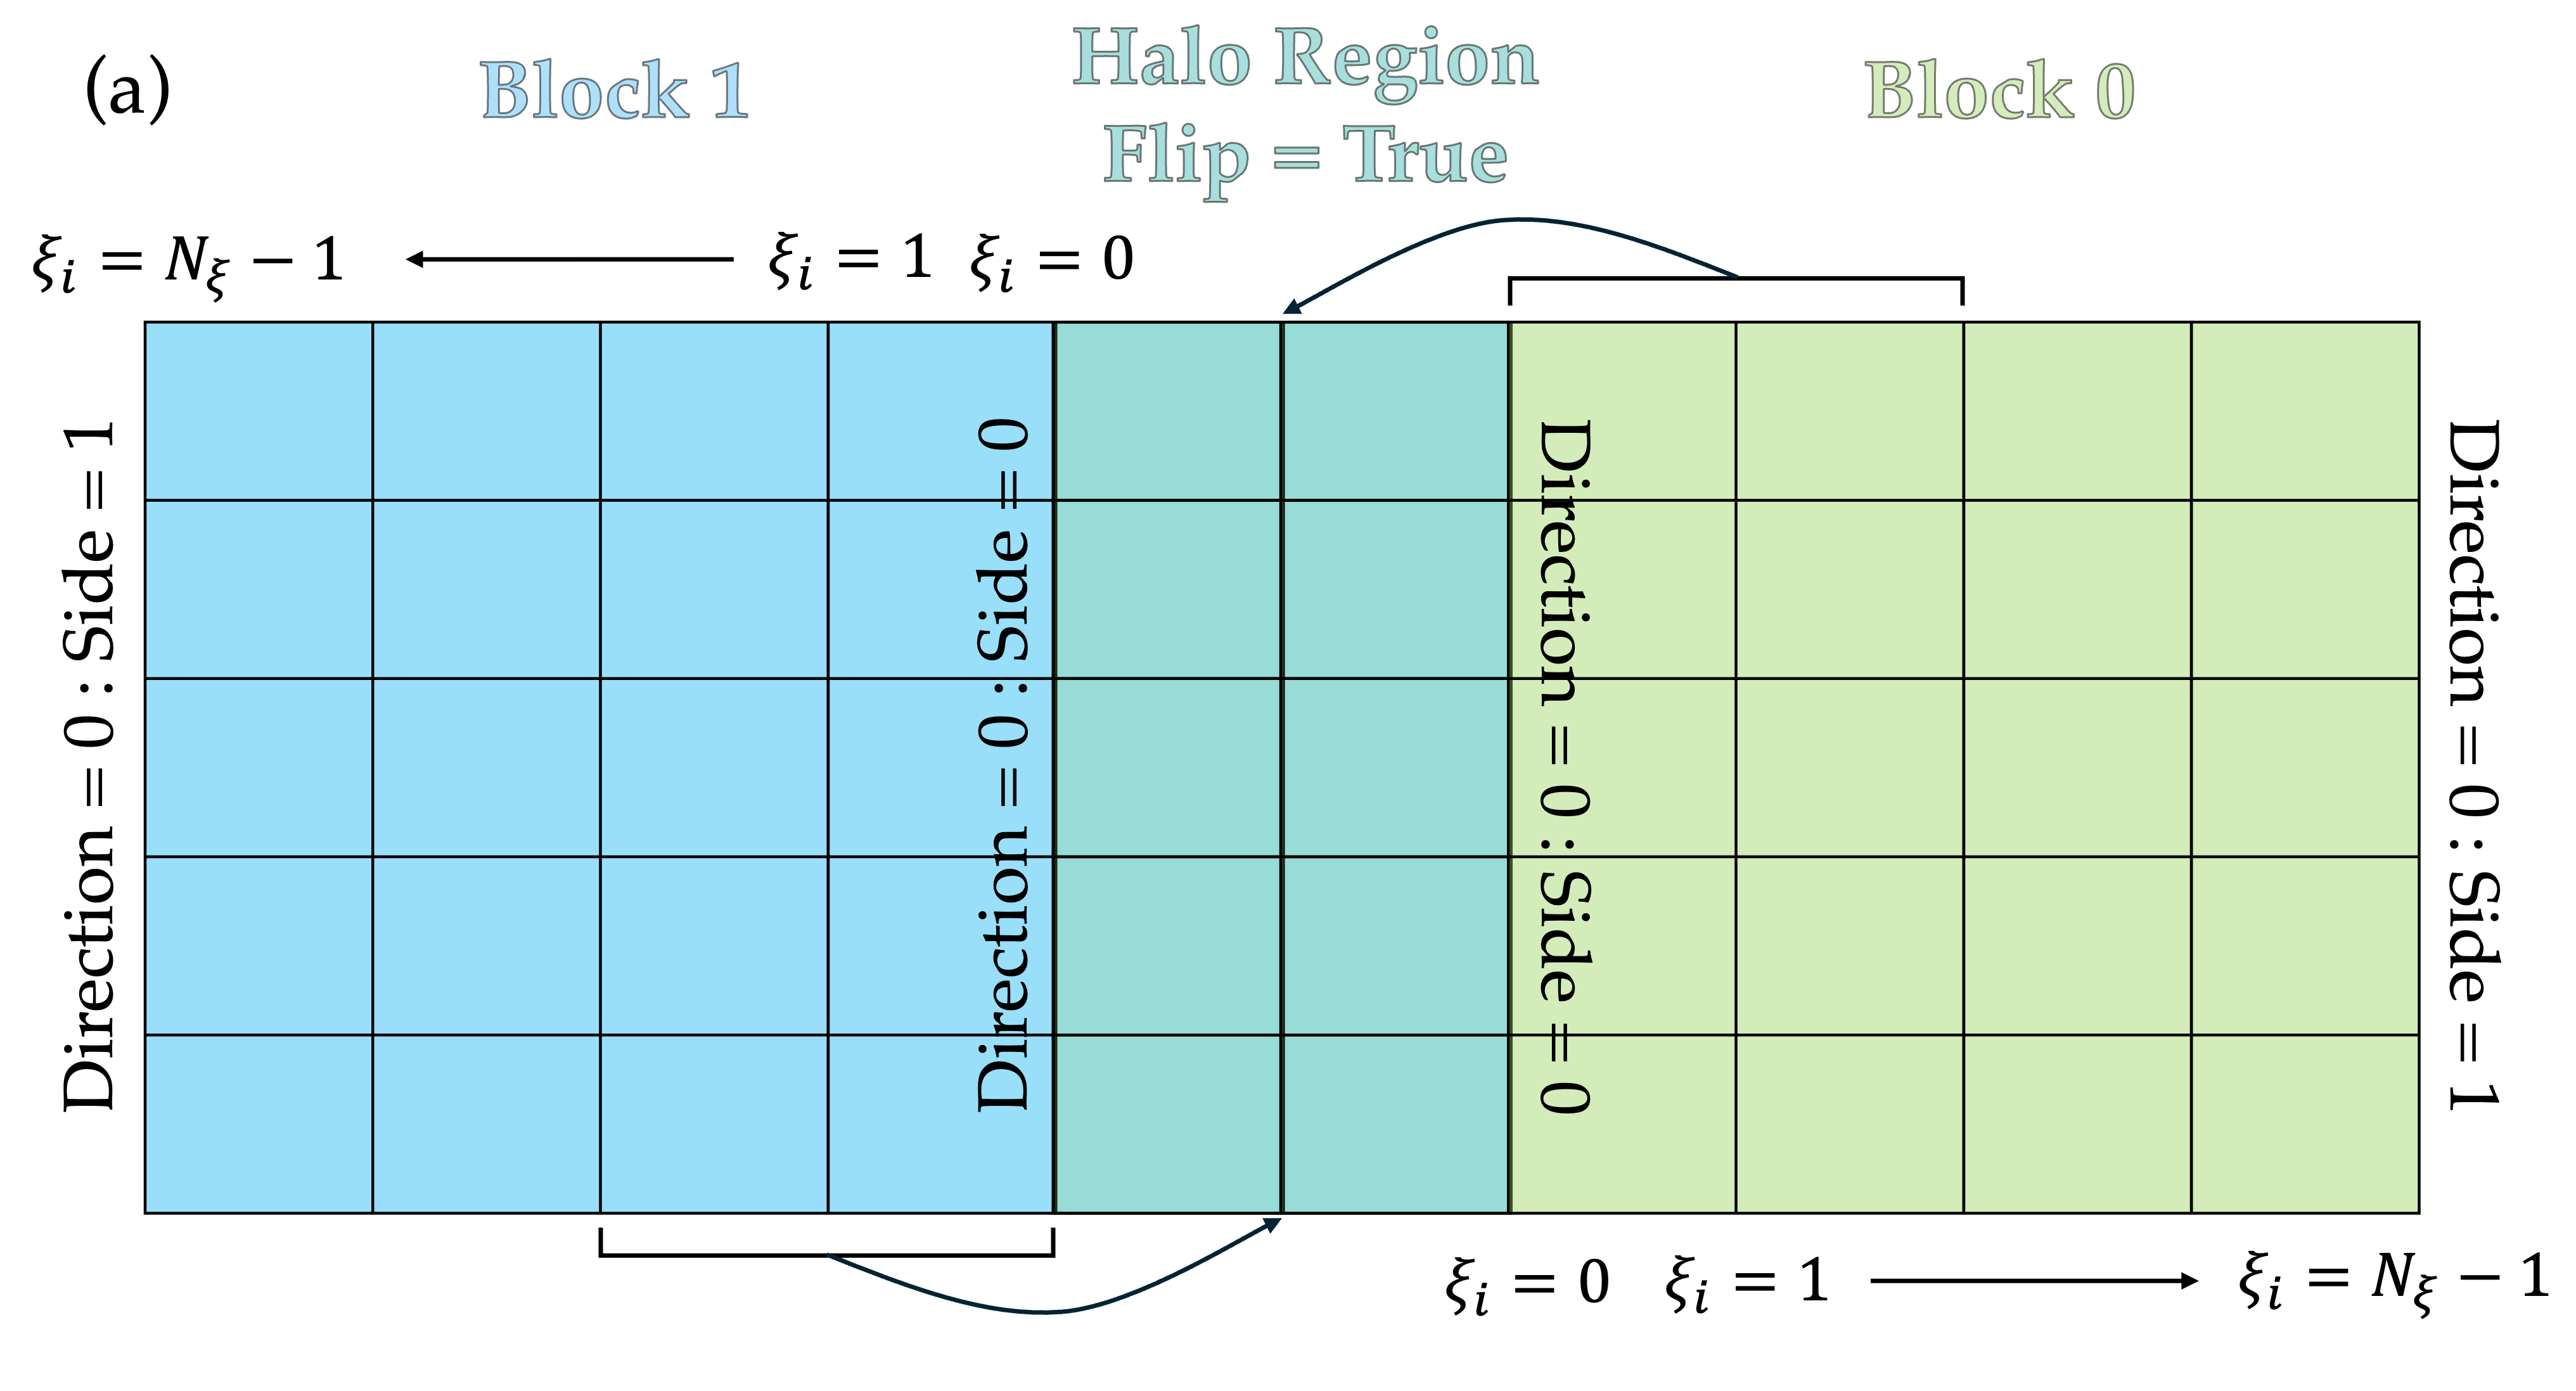
\includegraphics[width=0.495\textwidth]{./images/OpenSBLI_MB_B0_B1}
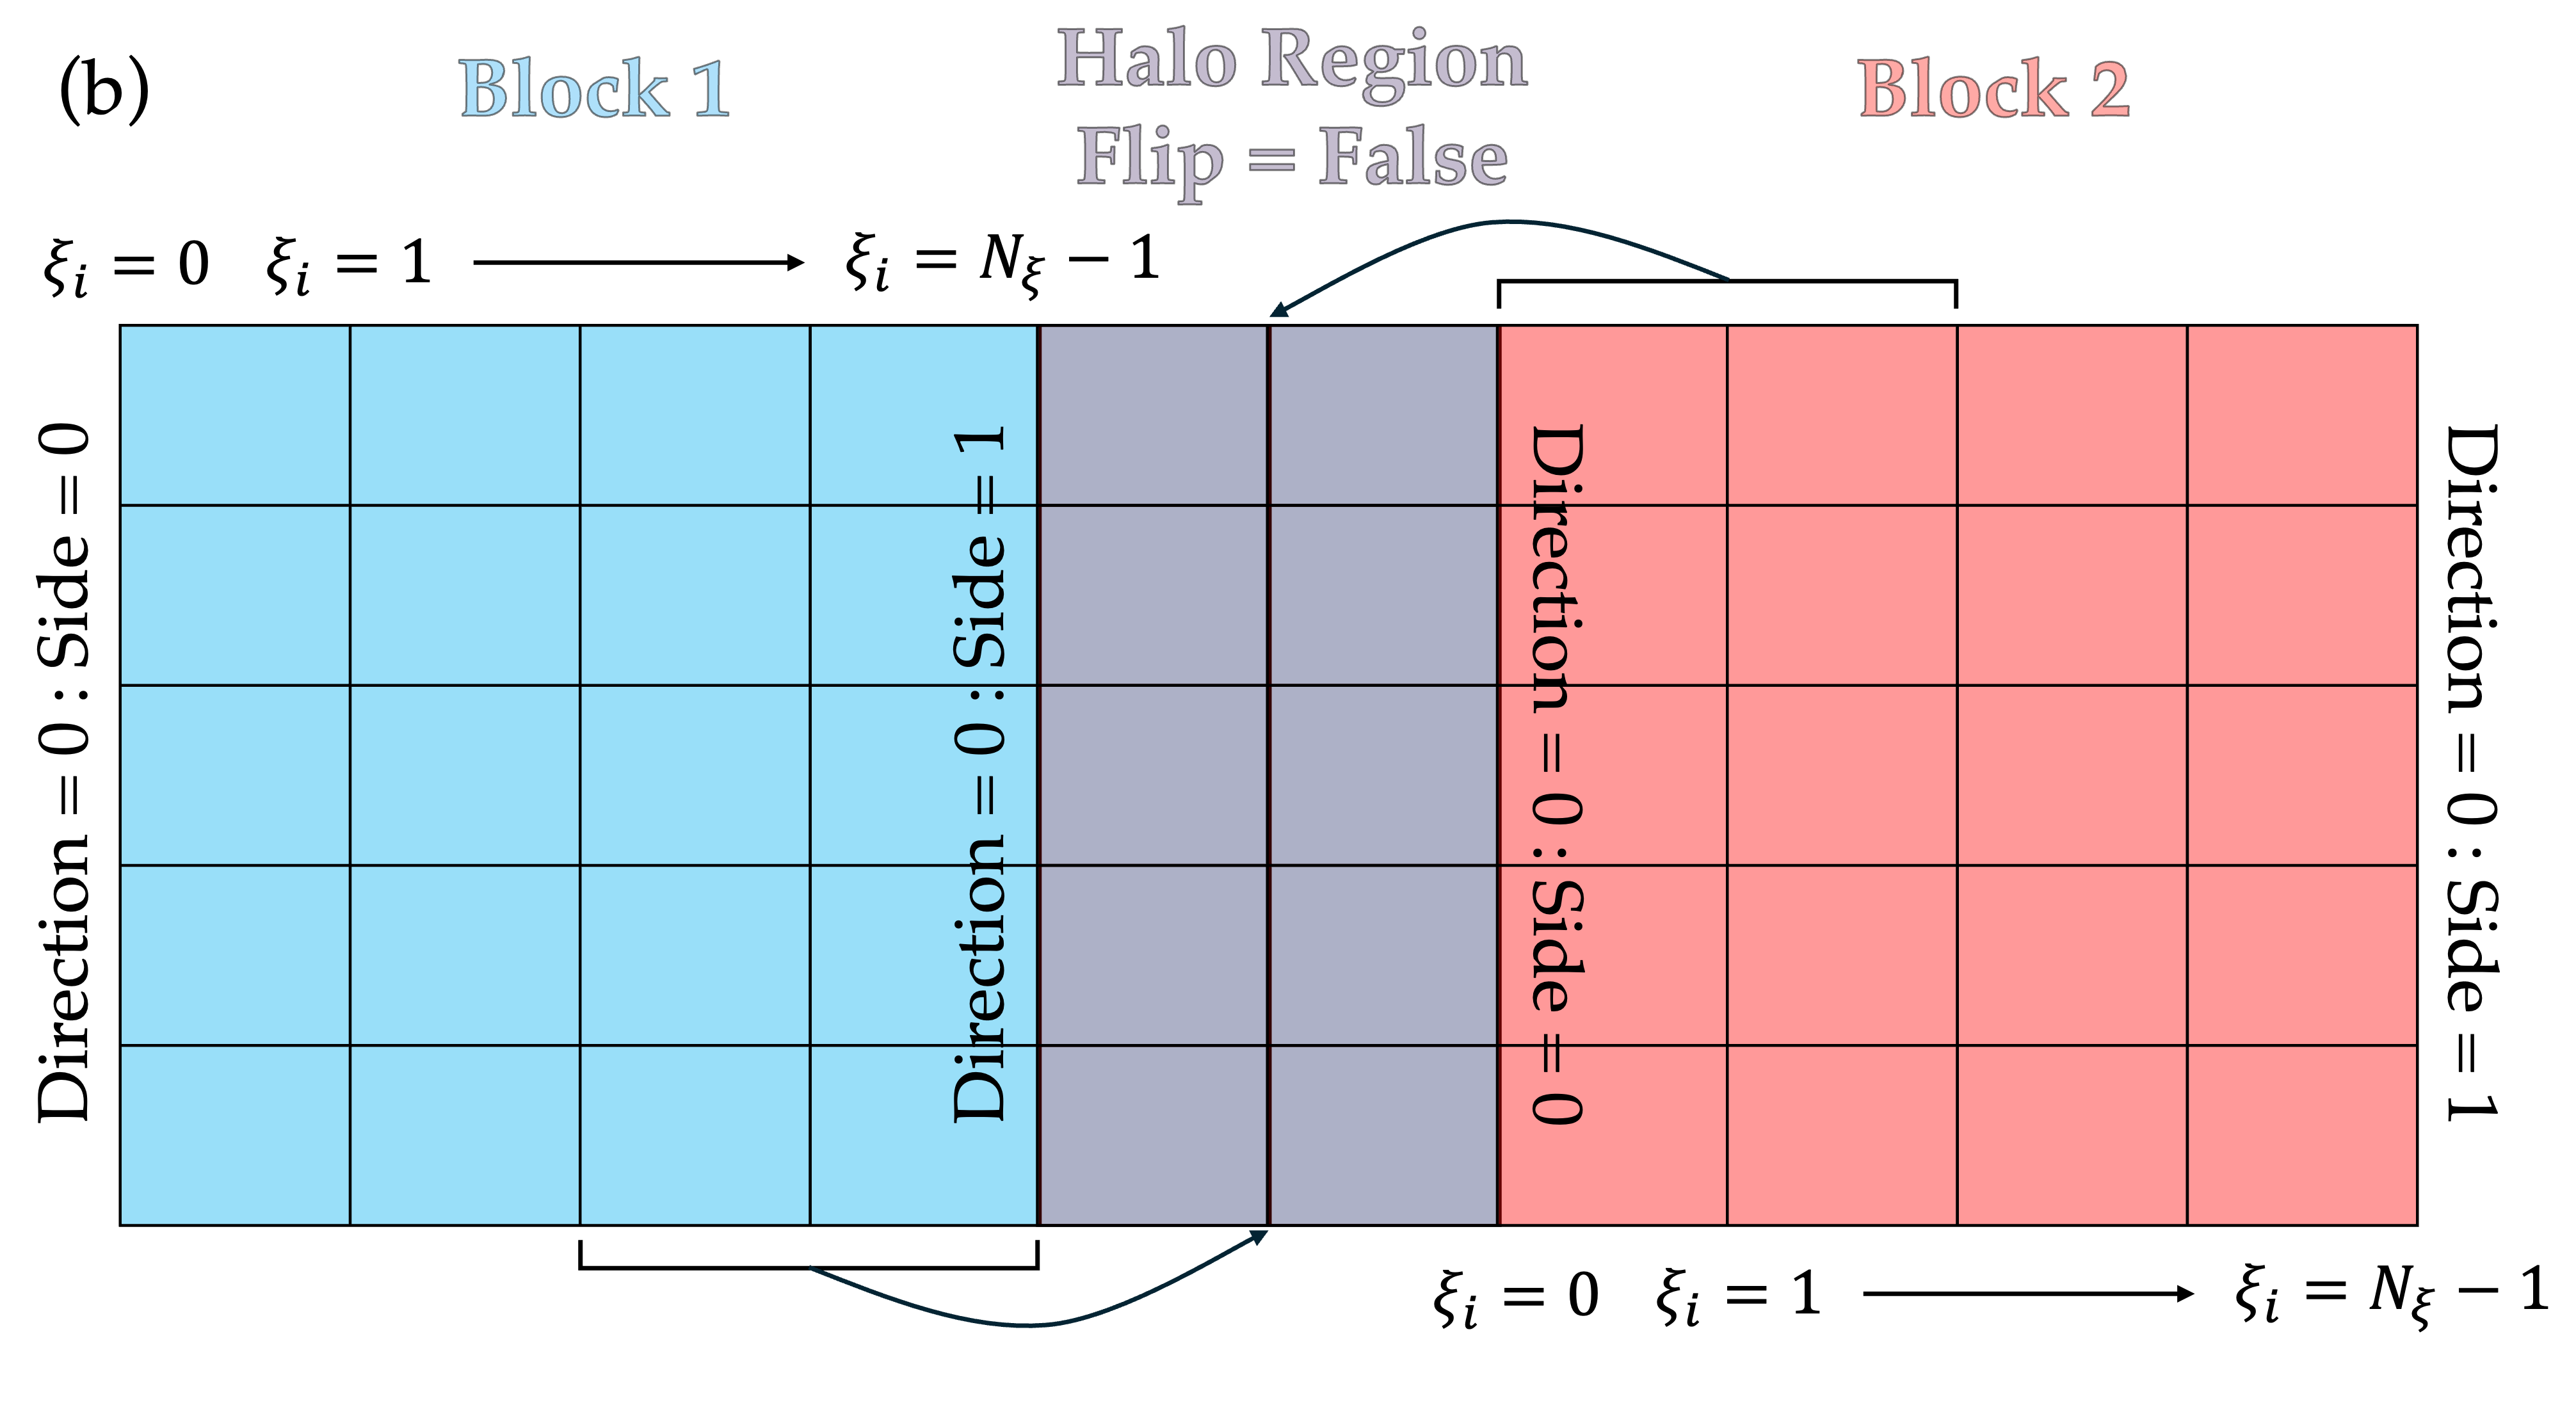
\includegraphics[width=0.495\textwidth]{./images/OpenSBLI_MB_B1_B2}
\caption{Example multi-block interface schematic corresponding to the block layout in Figure~\ref{fig:mesh_blocks}. Showing matching block interfaces with indices (a) increasing in opposite directions from the interface (Flip=True), and (b) in the same direction (Flip=False). Data is exchanged from the start/end of each block to the halo region of the matching block.}
\label{fig:MB_schematic}
\end{center}
\end{figure}

 When defining a multi-block problem, it is essential to specify interface conditions to instruct OpenSBLI how the blocks are arranged relative to one another. This is achieved by defining \verb|InterfaceBC| boundary conditions. Referring to the aerofoil mesh in Figure~\ref{fig:mesh_blocks}, we have: wake block 0 (green), aerofoil block 1 (blue), and wake block 2 (red).

 \begin{lstlisting}
 # Specify an interface condition on block 1, at the interface with block 0 (bottom wake block)
InterfaceBC(direction=0, side=0, halos=[-2,2], name="block1_to_block0", match=(0, 0, 0, True))
# Specify an interface condition on block 1, at the interface with block 2 (top wake block)
InterfaceBC(direction=0, side=1, halos=[-2,2], name="block1_to_block2", match=(2, 0, 0, False))
\end{lstlisting}

In the example above and schematic in Figure~\ref{fig:MB_schematic}, the interface connections for the aerofoil mesh (block 1) to the wake blocks (block 0, block 2) are defined. The first two inputs to \verb|InterfaceBC| are the direction (0, 1, 2) and side (0, 1), as is standard with all boundary conditions in OpenSBLI. The example here is setting the boundaries for the $(\xi, 0)$ direction for the coordinate around the aerofoil, which starts at the trailing edge on the lower side ($i=0$) and ends at the trailing edge on the upper side ($i=N_\xi - 1$). The halo depth for the swaps can be specified, along with a name for the exchange computation. The part that interfaces with other blocks is controlled by the \verb|match| parameter. The \verb|match| parameter specifies the other block to connect to. The syntax is \verb|match = (block number, direction, side, flip)|. In line 2 of the example above, the aerofoil block is connected to block 0, in the $(\xi, 0)$ direction on its side 0. In line 4, the aerofoil block is connected to block 2, in the $(\xi, 0)$ direction on its side 0.

Referring to the indexing shown in the schematic in Figure~\ref{fig:MB_schematic}, the boolean parameter \verb|flip| instructs OpenSBLI whether to flip the block index when making the swaps. This depends on the mesh generation, the indexing convention selected, and how the user has defined the problem. For the aerofoil example, both wake blocks are indexed in $\xi$ starting from the trailing edge at $i=0$, and ending at the outflow at $i=N_\xi-1$. However, the upper aerofoil-block interface matches the final index of the aerofoil block ($i=N_\xi - 1$) to the start of the wake block ($i=0$), but the lower aerofoil-block interface matches the start of the aerofoil block ($i=0$) with the start of the wake block ($i=0$). This requires the lower interface to pass \verb|flip=True| to flip the orientation of the swaps, as the index increases $i=0, 1, 2, \dots$ in opposite directions in that case. These interface boundaries are set amongst the other regular boundary conditions (e.g. no-slip wall, far-field, outlet), and set on the \verb|MultiBlock| class using the \verb|set_block_boundaries| as in OpenSBLI v2.0.

\newpage
\section{Example governing equations}

\subsection{Central schemes with skew-symmetric formulation}\label{sec:central_skew}
An example of the compressible Navier-Stokes equations written in skew-symmetric form to improve stability. An alternative skew formulation can be found in the turbulent channel flow application. 
\begin{lstlisting}
# Define the compresible Navier-Stokes equations in Einstein notation, by default the scheme is Central no need to
mass = "Eq(Der(rho,t), - Skew(rho*u_j,x_j))"
momentum = "Eq(Der(rhou_i,t) , - Skew(rhou_i*u_j, x_j) - Der(p,x_i)  + Der(tau_i_j,x_j))"
energy = "Eq(Der(rhoE,t), - Skew(rhoE*u_j,x_j) - Conservative(p*u_j,x_j) + Der(q_j,x_j) + Der(u_i*tau_i_j ,x_j))"
# Substitutions used in the equations
stress_tensor = "Eq(tau_i_j, (mu/Re)*(Der(u_i,x_j)+ Der(u_j,x_i)- (2/3)* KD(_i,_j)* Der(u_k,x_k)))"
heat_flux = "Eq(q_j, (mu/((gama-1)*Minf*Minf*Pr*Re))*Der(T,x_j))"
substitutions = [stress_tensor, heat_flux]
# Constants that are used
constants = ["Re", "Pr", "gama", "Minf"]
# symbol for the coordinate system in the equations
coordinate_symbol = "x"
# Constituent relations used in the system
velocity = "Eq(u_i, rhou_i/rho)"
pressure = "Eq(p, (gama-1)*(rhoE - rho*(1/2)*(KD(_i,_j)*u_i*u_j)))"
temperature = "Eq(T, p*gama*Minf*Minf/(rho))"
viscosity = "Eq(mu, 1.0)" # Note: constant viscosity here
\end{lstlisting}

\subsection{General implementation of different Navier-Stokes split forms for Central schemes}
The example above shows manual specification of the Navier-Stokes equations in a split form. In OpenSBLI V3, a general class has been added with several different quadratic- and cubic-split forms. The usage is shown below. Note this replaces manual specification of the equations, and is only for usage with either pure central difference schemes or central schemes to be used in conjunction with the WENO filter step method.

\begin{lstlisting}
coordinate_symbol = "x"
constants = ["Re", "Pr", "gama", "Minf", "SuthT", "RefT"]
NS = NS_Split('KGP', ndim, constants, coordinate_symbol=coordinate_symbol, viscosity='dynamic', energy_formulation='enthalpy', debug=False)
mass, momentum, energy = NS.mass, NS.momentum, NS.energy
# Expand the simulation equations, for this create the simulation equations
simulation_eq = SimulationEquations()
simulation_eq.add_equations(mass)
simulation_eq.add_equations(momentum)
simulation_eq.add_equations(energy)
\end{lstlisting}

The equations returned from the \verb|NS_Split| class can be modified before being added to the \verb|SimulationEquations| class. the \verb|viscosity| option can either be set to \verb|'constant'| or \verb|'dynamic'|. In the case of dynamic viscosity, an expression for $\mu$ must be given to the constituent relations class. Certain schemes have different options to apply to splitting of the energy equation. In this example, the \verb|KGP| cubic-split form is selected with the energy equation split on enthalpy. For this, enthalpy must also be defined as a constituent relation by the user. Currently, the following schemes are available: \verb|Divergence|, \verb|Blaisdell|, \verb|Jameson|, \verb|Feiereisen|, \verb|Kok|, \verb|KGP|, \verb|KEEP|. 

\subsection{Shock capturing schemes in conservative form}
An example of using the shock capturing schemes with the Navier-Stokes equations written in conservative form. Dynamic viscosity is being evaluated with Sutherland's law. Alternatively a power law could be used here. Note that the speed of sound must be specified as a constituent relation for the characteristic decomposition.
\begin{lstlisting}
sc1 = "**{\'scheme\':\'Teno\'}"
# Define the compresible Navier-Stokes equations in Einstein notation.
mass = "Eq(Der(rho,t), - Conservative(rhou_j,x_j,%s))" % sc1
momentum = "Eq(Der(rhou_i,t) , -Conservative(rhou_i*u_j + KD(_i,_j)*p,x_j , %s) + Der(tau_i_j,x_j) )" % sc1
energy = "Eq(Der(rhoE,t), - Conservative((p+rhoE)*u_j,x_j, %s) - Der(q_j,x_j) + Der(u_i*tau_i_j ,x_j) )" % sc1
stress_tensor = "Eq(tau_i_j, (mu/Re)*(Der(u_i,x_j)+ Der(u_j,x_i) - (2/3)* KD(_i,_j)* Der(u_k,x_k)))"
heat_flux = "Eq(q_j, (-mu/((gama-1)*Minf*Minf*Pr*Re))*Der(T,x_j))"
# Substitutions
substitutions = [stress_tensor, heat_flux]
constants = ["Re", "Pr", "gama", "Minf", "SuthT", "RefT"]
# Define coordinate direction symbol (x) this will be x_i, x_j, x_k
coordinate_symbol = "x"
# Formulas for the variables used in the equations
velocity = "Eq(u_i, rhou_i/rho)"
pressure = "Eq(p, (gama-1)*(rhoE - rho*(1/2)*(KD(_i,_j)*u_i*u_j)))"
speed_of_sound = "Eq(a, (gama*p/rho)**0.5)"
temperature = "Eq(T, p*gama*Minf*Minf/(rho))"
viscosity = "Eq(mu, (T**(1.5)*(1.0+SuthT/RefT)/(T+SuthT/RefT)))"
\end{lstlisting}

\newpage
\section{Monitoring quantities during the simulation}
OpenSBLI has a \textit{SimulationMonitor} class to print output of point values (data probes) during a simulation if required. The output displays the current simulation time, iteration number, and a series of column data for each of the probes, printed at a given iteration frequency. The simulation monitor class can be added to a problem script as follows.

\begin{lstlisting}
arrays = ['u0', 'p']
arrays = [block.location_dataset('%s' % dset) for dset in arrays]
indices = [('block0np0/2', 'block0np1/2', 0), ('block0np0/2', 'block0np1/2', 0)]
SM = SimulationMonitor(arrays, indices, block, print_frequency=250, fp_precision=12, output_file='output.log')
alg = TraditionalAlgorithmRK(block, simulation_monitor=SM)
\end{lstlisting}

In this example there are two probes, one for streamwise velocity, and one for pressure. Each quantity has a corresponding grid location $\left(i, j, k\right)$, given as a tuple in line 3. The grid indices can either be given as integers or as factors of the total grid points in each direction (block0np0, block0np1, block0np2). The simulation monitor is added to the algorithm in the final line and will appear at the end of the time-loop in the generated C code. The input options are:

\begin{enumerate}
\item{\textbf{arrays:} The physical quantities to be monitored. These can be any array defined within the simulation.}
\item{\textbf{indices:} The $\left(i, j, k\right)$ grid indices for the probe's location.}
\item{\textbf{block:} An OpenSBLI simulation block.}
\item{\textbf{print\_frequency:} The desired printing frequency.}
\item{\textbf{fp\_precision:} Floating point precision of the output.}
\item{\textbf{output\_file:} Name of the log file. If this argument is not provided, the output is printed to standard out.}
\end{enumerate}

\newpage
\section{Reduced dimension data operations}
Often while running large simulations to generate unsteady data, regularly writing out the full-3D flowfield is unfeasible. In OpenSBLI V3.0, new features of the OPS library are now supported. These enable the output of reduced dimension data, and the ability to perform partial reductions over individual dimensions individaully.

\subsection{Generating 2D slice output to disk}
Specification of the new I/O slicing class is shown below.
\begin{lstlisting}
# Block 1 slicing (aerofoil block)
grid_slice = iohdf5_slices(blocknumber=1, **{'iotype': "Init"})
coords = [([DataObject('x0'), DataObject('x1')], 2, 'block1np2/2')]
grid_slice.add_slices(coords)
# Q vector slices written out in time
q_slice = iohdf5_slices(save_every=500, blocknumber=1, **{'iotype': "Write"})
# x-y side view
slices = [(q_vector, 2, 'block1np2/2')]
# Aerofoil surface
slices += [(q_vector, 1, 1)]
q_slice.add_slices(slices)
# Set both HDF5 output objects
multi_block.setio([grid_slice, q_slice])
\end{lstlisting}
The \verb|iohdf5_slices| class is used in a similar way to the regular \verb|iohdf5| class. However, the slicing class only supports output of data, and does not read data into the simulation. The \verb|iotype| can either be \verb|Init| to output once at the start of the simulation, or \verb|Write|, to output data at a set iteration frequency (\verb|save_every|) during the time loop. The user must provide a tuple containing the arrays to output, the direction in which to orient the slice, and the grid index for that slice location. For example, \verb|(q_vector, 1, 1)| outputs a slice of the conservative variables in the $x_1$ direction, on the $j=1$ index. As with other classes, for multi-block problems, different slicing options can be selected on different blocks independently using the \verb|blocknumber| input parameter.

\subsection{Partial dimensionality reductions during the run}
Many of the 3D simulations will have one or more periodic direction. Users may want to perform a spatial average over this direction at regular time intervals. Previously, the full-3D flowfield had to be written out to disk and this operation was performed external to the simulation. However, for large mesh sizes this is not feasible. Users can now perform partial reductions along individual dimensions during the run. Currently, this should be added directly to the C/C++ code by the user depending on their requirements. An example parallel region and corresponding kernel code are given below for a 3D to 2D operation.

\begin{lstlisting}
ops_par_loop(reduct22D, "reduct22D", block, 3, range_3D,
ops_arg_dat(dat3D, 1, S3D_000, "double", OPS_READ),
ops_arg_dat(dat2D_XY, 1, S3D_000_STRIDE3D_XY, "double", OPS_INC));
\end{lstlisting}
The kernel takes a 3D dataset as an \verb|OPS_READ| input (\verb|dat3D|), with a 3D stencil \verb|S3D_000|. An \verb|OPS_INC| summation operation is performed over a strided stencil \verb|S3D_000_STRIDE3D_XY|. The strided stencil in this case is defined to perform a summation over the $z$ direction as 
\begin{lstlisting}
// Strided stencil for xy direction
int stride3D_xy[] = {1,1,0};
int s3D_000[] = {0, 0, 0};
ops_stencil S3D_000_STRIDE3D_XY = ops_decl_strided_stencil(3, 1, s3D_000, stride3D_xy, "s2D_000_stride3D_xy");
\end{lstlisting}
This parallel region and strided stencil are combined with the kernel shown below to perform the partial reduction from a 3D array to a span-averaged 2D array. Multiple arrays can be span-averaged within the same kernel. If this operation happens multiple times, a second kernel must be specified beforehand to zero the 2D arrays prior to performing the partial reductions. Reductions to 1D arrays are also supported in the case of doubly periodic configurations.
\begin{lstlisting}
void reduct22D(const ACC<double> &dat3D, ACC<double> &dat2D_xy)
{
dat2D_xy.combine_inc(0,0,0,dat3D(0,0,0));
}
\end{lstlisting}

\newpage
\section{Generation of post-processing kernels and reduction objects}
Previously, post-processing kernels to extract physical quantities not present in the governing equations needed to be added manually to the C code. In OpenSBLI V3.0, they can now be specified in the Python front-end and combined with new reduction operator data objects. An example of volume integrated quantities for the supersonic Taylor-Green vortex case is shown below.
\begin{lstlisting}
# Define symbolic quantities
vel = symbols("u0:%d"%ndim,  **{'cls':DataObject})
wx, wy, wz = symbols("wx wy wz",  **{'cls':GridVariable})
coords = symbols("x0:%d"%ndim,  **{'cls':CoordinateObject})
# Matrix of derivatives
M = Matrix(ndim,ndim,[CD(u,x) for u in vel for x in coords])
# Post-processing class
post = UserDefinedEquations(computation_name='TGV post-process')
post.algorithm_place = InTheSimulation(frequency=100)
# Define vorticity and dilatation components
vortx = Eq(wx, M[2,1] - M[1,2])
vorty = Eq(wy, M[0,2] - M[2,0])
vortz = Eq(wz, M[1,0] - M[0,1])
dil = Eq(DataObject('divV'), M[0,0] + M[1,1] + M[2,2])
\end{lstlisting}
A \verb|UserDefinedEquations| class is instantiated, to be executed within the main time loop using the \verb|InTheSimulation| algorithm placement selector. The equations will be evaluated at the user chosen iteration count of 100 specified by the \verb|frequency| argument. The property \verb|order| can also be added to this class to fine tune the position of the kernel execution within the main placeholder.

The new reduction operator objects are: \verb|ReductionSum|, \verb|ReductionMin|, and \verb|ReductionMax|, for performing summation and minimum/maximum reductions in the C/C++ code. These can now be specified within the symbolic equations in the Python front-end. Example usage is shown below.
\begin{lstlisting}
# Define reduction quantities
rho_m, KE_m, eps_D, eps_S = symbols('rhom KE eps_D eps_S', **{'cls':ReductionSum})
# Build the summation equations
rho_eqn = OpenSBLIEq(rho_m, rho_m + DataObject('rho'))
ke_eqn = OpenSBLIEq(KE_m, KE_m + 0.5*DataObject('rho')*sum([u**2 for u in vel]))
dilatation_eqn = OpenSBLIEq(eps_D, eps_D + Rational(4,3)*DataObject('mu')*divV**2)
enstrophy_eqn = OpenSBLIEq(eps_S, eps_S + DataObject('mu')*(wx**2 + wy**2 + wz**2))
# Add to the post-process class
post.add_equations([vortx, vorty, vortz, dil, rho_eqn, ke_eqn, dilatation_eqn, enstrophy_eqn])
\end{lstlisting}
If reduction operators are present within the equations, OpenSBLI will automatically define all of the OPS constructs and loops required to perform the parallel reduction. In this case, a sum is performed over the volume. These quantites can be added to the \verb|SimulationMonitor| class to generate text column outputs of the data at the requested iteration frequency.

\newpage
\section{Specification of reduced- and mixed-precision}
The code-generation interface can also be used to select the precision of the simulation code. The supported options are \verb|Double|, \verb|FloatC| (single) and \verb|Half|.

\begin{lstlisting}
# Set the global simulation precision to single
SimulationDataType.set_datatype(FloatC)
# Define custom mixed-precision options using presets
mixed_precision_config = {
'q_vector' : ([], Double),
'RK_arrays' : ([], Double),
'residuals' : ([], FloatC),
'wk_arrays' : ([], FloatC),
'casting' : 'explicit'}
# Optionally, select custom arrays to set the precision of
custom_arrays = [block.location_dataset(dset) for dset in ['T', 'p']]
mixed_precision_config['custom'] = (custom_arrays, Half)
# Call the OPS C code-generator 
OPSC(alg, mixed_precision_config)
\end{lstlisting}
In this example, a mixed-precision configuration is selected. The global simulation precision is set to single, with certain quantities kept at double precisiion. A few presets are available, to apply mixed precision to the time-advance arrays, Runge-Kutta time-stepping arrays, residuals of the RHS of the governing equations, or the temporary work arrays. Alternatively, the custom option allows the precision of any quantity to be raised or lowered relative to the global precision. In this case the temperature and pressure arrays are set to half precision.

\newpage
\section{Useful SymPy functions for OpenSBLI development}
To be able to develop new features for OpenSBLI, a good knowledge of Python and the SymPy library is required. The best resource is the SymPy online documentation: \url{https://docs.sympy.org/1.1/index.html}. Some commonly used functionality in OpenSBLI is listed here with examples.

\subsection{Pretty printing of equations: pprint}
At any point within the code generation process the user is able to take a list of symbolic equations and print them to screen to be checked. The best way to do this is with SymPy's \verb|pprint| function. Many of the classes in OpenSBLI will store equations as an \verb|equations| attribute to an object, which can be iterated over and printed to screen:
\begin{lstlisting}
from sympy import pprint
for equation in kernel.equations:
	pprint(equation)
\end{lstlisting}
The pretty print function can be used throughout the entire source-code and in the problem set up files.
\subsection{Creating symbolic objects: symbols}
There are three main ways of generating symbolic objects in OpenSBLI. The first is to simply call one of the OpenSBLI object classes with a string as a name:
\begin{lstlisting}
p = DataObject('p')
\end{lstlisting}
This creates a \verb|DataObject| which will later be converted into a \verb|DataSet| defined on a block. Note that the variable $p$ on the left hand side is simply a Python variable used to refer to this object during code generation, it has no effect on the output code. The name passed to the \verb|DataObject| class as a string will be written out in the simulation code, so ensure that this variable has been defined elsewhere in the script. If you have already created a \verb|SimulationBlock| you can create a \verb|DataSet| directly on that block with:
\begin{lstlisting}
p = block.location_dataset('p')
pprint(p)
p_B0[0,0,0]
\end{lstlisting}
Note that the DataSet has indices as it is an indexed object with $i$ indices for the $i$ number of dimensions in the problem. The \verb|DataSet| has also been given a `\_B0' suffix to denote that it is defined on a block numbered 0. The third method is a quick way to create several symbols of the same type using the \verb|symbols| class of SymPy.
\begin{lstlisting}
p, u, v, w = symbols('p u v w', **{'cls': DataObject})
\end{lstlisting}
The type of object created here could be \verb|DataObject, GridVariable| or \verb|ConstantObject| depending on the application.

\subsection{Off-setting an indexed object}
OPS uses a stencil-based approach for data access. As the \verb|ops_par_loop| iterates over the discrete grid points, the current grid point being evaluated is always denoted as [0,0,0] in three dimensions. To build finite-difference approximations we need the ability to access data that is offset from the [0,0,0] location. OpenSBLI contains a function to let users index DataSets for a given number of grid points away from the current location in a certain direction. For example to index the above DataSet in the $i=1$ dimension by three grid points:

\begin{lstlisting}
from opensbli.utilities.helperfunctions import increment_dataset
p = block.location_dataset('p')
pprint(p)
p_B0[0,0,0] # The base [0,0,0] location for a generic stencil
direction, increment = 1, 3 # index direction 1 by 3 grid points
p_shifted = increment_dataset(p, direction, increment)
pprint(p_shifted)
p_B0[0,3,0]
\end{lstlisting}
This functionality is frequently used when developing numerical schemes or boundary conditions, where the expression requires data offset from the current [0,0,0] grid point. For example to create a \nth{4} order central difference approximation for a given direction, the user would create a list [-2, -1, 1, 2] and build the finite-difference approximation by looping over the offsets with four applications of the \verb|increment_dataset| function.

\subsection{Substitution of symbolic quantities}
SymPy has various methods for substituting terms into existing symbolic expressions. Most of these rely on setting up either a Python dictionary or tuples to create pairs of the existing terms and the new term to be substituted in to the expression. An example with the \verb|replace| function would be:
\begin{lstlisting}
for old, new in zip(to_be_replaced, new_terms):
    term = term.replace(old, new)
\end{lstlisting}
Alternatively the SymPy function \verb|subs| can be used with a substitution dictionary containing \verb|{key: value}| pairs such that:
\begin{lstlisting}
expression.subs(substitution_dictionary)
\end{lstlisting}
Always \verb|pprint| the expression before and after the substitution to check that you are getting the correct behaviour. Sometimes for more complex expressions multiple applications of the substitution functions will be required.

\subsection{Left and right hand sides of equations}
When manipulating equations in OpenSBLI, the user will often need to access the left and right hand sides of an equation (of type \verb|Eq|) individually. This is true for the substitutions in the previous section, where it is often the right hand side of an equation that needs to be modified. The left and right hand sides of an equation can be accessed simply with:

\begin{lstlisting}
print(example_equation)
Eq(p, (gama - 1)*(-rho*u0**2/2 - rho*u1**2/2 - rho*u2**2/2 + rhoE))
print(example_equation.lhs)
p
print(example_equation.rhs)
(gama - 1)*(-rho*u0**2/2 - rho*u1**2/2 - rho*u2**2/2 + rhoE)
\end{lstlisting}

\subsection{De-nesting multiple iterables}
Often in OpenSBLI you will encounter iterables that contain iterables. A common example of this would be a list of lists in Python. To be able to iterate over all of the individual items directly in a single loop it is often convenient to use the SymPy function \verb|flatten|. This function collapses the list of list structure into a single list containing all of the items to iterate over.
\begin{lstlisting}
>>> from sympy import flatten
>>> x = [[1, 2, 3], [4, 5,6]]
>>> print(x)
[[1, 2, 3], [4, 5, 6]]
>>> print(flatten(x))
[1, 2, 3, 4, 5, 6]
\end{lstlisting}

\subsection{Accessing attributes in Python objects: \_\_dict\_\_}

All objects in Python have a \verb|.__dict__| routine to show the attributes contained in that object. This is frequently used when developing features for OpenSBLI. The \verb|.__dict__| routine returns a Python dictionary \verb|{key: value}| pair. For example, in an OpenSBLI \verb|Kernel| class the equations defined in that kernel will be stored and can be accessed in the attribute \verb|kernel.equations|. In the code snippet below the \verb|.__dict__| function is showing the attributes defined in the Runge-Kutta time-stepping class after it has been instantiated.

\begin{lstlisting}
>>> rk = RungeKutta(3)
>>> print(rk.__dict__)
{'solution_coeffs': rkold[stage], 'stage_coeffs': rknew[stage], 'name': 'RungeKutta', 'iteration_number': iter, 'temporal_iteration': iter, 'solution': {}, 'schemetype': 'Temporal', 'constant_time_step': True, 'time_step': dt, 'order': 3, 'nloops': 2, 'stage': stage}
\end{lstlisting}


\subsection{Using built-in SymPy functions (sin, cos, exp, ...)}
It's important to understand the differences between the common mathematics functions that are available in Python. In the majority of cases for OpenSBLI, common math functions should be imported from the symbolic SymPy library. A common mistake is to use either the Python \verb|math| library or \verb|NumPy|. Both of these will throw errors when trying to build symbolic expressions in OpenSBLI.
\begin{lstlisting}
>>> import math, numpy, sympy
>>> print([math.cos(0.5), numpy.cos(0.5), sympy.cos(0.5)])
[0.8775825618903728, 0.8775825618903728, 0.877582561890373]
>>> x = sympy.symbols('x')
>>> sympy.cos(x)
cos(x)
>>> math.cos(x)
Traceback (most recent call last):
    raise TypeError("can't convert expression to float")
TypeError: "can't convert expression to float"
\end{lstlisting}
Sometimes it can be useful to ask SymPy not to evaluate numerical expressions, or explicitly use symbolic expressions in a function:
\begin{lstlisting}
>>> sympy.cos(0.5)
0.877582561890373
>>> sympy.cos(0.5, evaluate=False)
cos(0.5)
>>> sympy.cos(sympy.Rational(1,2))
cos(1/2)
\end{lstlisting}
Other common mathematical functions in SymPy can be used in OpenSBLI, which will be converted into C code at the code generation stage. Examples include \verb|Abs, Min, Max, ceil|.

\subsection{Conditional expressions (if-else branching)}\label{sec:piecewise}
SymPy also has a boolean logic system that allows us to symbolically create branching if-else statements in the C code. A simple conditional function such as
\[
    \rho= 
\begin{cases}
    10,& \text{if } x < 3\\
    5,& \text{if } x \geq 5\\
    0,              & \text{otherwise}
\end{cases}
\]
would be defined in OpenSBLI using SymPy's \verb|Piecewise| function as:
\begin{lstlisting}
x = DataObject('x0')
eqn = Eq(DataObject('rho'), Piecewise((10.0, x<3), (5.0, x>=5), (0.0,True)))
\end{lstlisting}
Each \verb|(value, condition)| tuple pair will be written out as branching if and else-if statements. The \verb|(value, True)| tuple is evaluated if all of the other conditions are not met in the simulation code. The Piecewise function will throw an error if an else statement is not provided in this format. More sophisticated conditional expressions can be built up using the SymPy \verb|And, Or| and \verb|Equality| classes. Each of these logic functions will be translated to the C equivalent in the final code.

OpenSBLI also has a \verb|GroupedPiecewise| class derived from the base SymPy version. GroupedPiecewise is useful when multiple equations are to be evaluated inside one of the conditional branches. Usage can be found for example in the \verb|teno.py| file. Tuple pairs of values and conditions can be built up using SymPy's \verb|ExprCondPair| class to be used to form a set of branching statements. Note that SymPy will simplify conditional logic if possible so you may not see every condition entered into the function.

\subsection{String representation: srepr}
Often it is useful to find out how SymPy is storing the symbolic quantities through its string representation functionality. The function \verb|srepr| breaks an expression down into its individual components and can be useful for debugging purposes. For example the pressure evaluation 
\begin{equation}
p = \left(\gamma -1\right) \left(\frac{u_{0}^{2}}{2} + \frac{u_{1}^{2}}{2} + \frac{u_{2}^{2}}{2} + \rho E\right)
\end{equation}
Has the string representation of:
\begin{lstlisting}
OpenSBLIEquation(DataObject('p'), Mul(Add(ConstantObject('gama'), Integer(-1)), Add(Mul(Integer(-1), Rational(1, 2), DataObject('rho'), Pow(DataObject('u0'), Integer(2))), Mul(Integer(-1), Rational(1, 2), DataObject('rho'), Pow(DataObject('u1'), Integer(2))), Mul(Integer(-1), Rational(1, 2), DataObject('rho'), Pow(DataObject('u2'), Integer(2))), DataObject('rhoE'))))
\end{lstlisting}
This is a good way of finding out which quantities are DataObjects, DataSets, ConstantObjects and GridVariables within an OpenSBLI expression. Finding the type of a single object can be done via the standard \verb|type()| function in Python.

\subsection{Breaking down an expression into its components: atoms/args}
Being able to manipulate symbolic expressions in OpenSBLI relies on knowing how to isolate certain components. Two useful functions within SymPy are \verb|atoms| and \verb|args|.

\begin{lstlisting}
>>> print(expression)
(gama - 1)*(-rho*u0**2/2 - rho*u1**2/2 - rho*u2**2/2 + rhoE)
>>> print(expression.atoms())
set([-1, -1/2, 2, gama, rho, rhoE, u0, u1, u2])
>>> print(expression.atoms(DataObject)))
set([rho, rhoE, u0, u1, u2])
>>> print(expression.atoms(ConstantObject))
set([gama])
\end{lstlisting}
A call to the \verb|atoms()| routine on any expression will return a set of symbolic quantities in it. This includes integers and rational constants. To extract a certain type of object from the expression to iterate over, an object type can be passed to atoms such as \verb|atoms(DataObject)|. Note that the output is a Python \verb|set|, which is an unordered collection of unique objects. These differ from a Python \verb|list|, which are an ordered collection that may contain duplicate entries. Useful operations can be performed on multiple sets such as \verb|intersection|, \verb|union| and \verb|difference|. These operations are often used in OpenSBLI to find all of the unique objects that have been defined throughout the code.


\begin{lstlisting}
# Take the right hand side of the continuity equation
>>> continuity_equation = simulation_eq.equations[0].rhs
>>> print(continuity_equation)
-CD rhou0_B0 x0 - CD rhou1_B0 x1 - CD rhou2_B0 x2
>>> print(continuity_equation.args)
(-CD rhou0_B0 x0, -CD rhou1_B0 x1, -CD rhou2_B0 x2)
# Take the first term d(rhou0)/dx
term = continuity_equation.args[0]
# Iterate over the components of the derivative operator
>>> print([x for x in term.args])
[-1, CD rhou0_B0 x0]
# Iterate over the derivative term
>>> derivative = term.args[1]
>>> print([x for x in derivative.args])
[rhou0_B0, x0]
\end{lstlisting}
The example above shows how to break down an expression into its individual terms and then isolate the individual components that make up those terms.


\subsection{Isolating terms of a certain type: isinstance}
The Python function \verb|isinstance| is frequently used to isolate objects of a certain type for modification. A use case for this would be if the user wanted to perform a modification only on a certain type of object in an expression while leaving the rest untouched. For example to modify only DataObjects in a given expression one could use:

\begin{lstlisting}
for term in equation.rhs.atoms():
    if isinstance(term, DataObject):
        # Perform some operation on the term
\end{lstlisting}

\subsection{Using GridVariables as temporary evaluations}
The purpose of the \verb|GridVariable| object is to evaluate a quantity locally for the current grid point, use it in an expression to set a \verb|DataSet| and then discard it. The \verb|GridVariable| will take different values at different grid points, but unlike a \verb|DataSet| it is not stored globally for later use. Examples of this are seen throughout OpenSBLI, for example in the definition of boundary conditions.

\subsection{Simplifying long expressions and reducing operation counts}
The final form of more complex expressions is not always the most efficient from a computational performance point of view. SymPy has a number of functions that can be used to try and simplify an expression in OpenSBLI. It is not always obvious which one is suitable (if any), without printing the expression before and after the modification. Among the possibilities for a given expression are:
\begin{enumerate}
\item{\verb|simplify(expression)|: Attempts to simplify an expression.}
\item{\verb|factor(expression)|: Attempts to factor polynomials.}
\item{\verb|horner(expression)|: Reduces a polynomial into a form requiring the minimum number of additions and multiplications by the Horner algorithm.}
\end{enumerate}

One method of assessing the impact of the attempted simplification is the \verb|count_ops()| routine. Using \verb|expression.count_ops()| gives the number of operations in the expression. This can be applied before and after one of the simplification methods to assess the output. Further methods for simplifying expressions can be found here: \url{https://docs.sympy.org/1.1/tutorial/simplification.html}.

\newpage
\section{HPC set-up on CSD3 NVIDIA P100 GPU machine}
These guidelines are for running OpenSBLI on the University of Cambridge `Service for Data Driven Discovery' (CSD3) system operated by the University of Cambridge Research Computing Service (\url{http://www.hpc.cam.ac.uk}), funded by EPSRC Tier-2 capital grant \textbf{EP/P020259/1}. The code runs on the NVIDIA P100 GPUs using the Intel compiler and OpenMPI for multi-GPU configurations.

\subsection{Example bashrc settings}
\begin{verbatim}
# Loading the necessary modules
module unload openmpi-1.10.7-gcc-5.4.0-jdc7f4f 
module unload gcc-5.4.0-gcc-4.8.5-fis24gg
module load intel/bundles/complib/2017.4
module unload intel/impi/2017.4/intel
module load openmpi-1.10.7-intel-17.0.4-exlc3jx
module load hdf5/openmpi-gdr/1.8.19
module unload hdf5/impi/1.8.16

# OPS specific library paths
export OPS_COMPILER=intel
export NV_ARCH=Pascal
export HDF5_INSTALL_PATH=/usr/local/Cluster-Apps/hdf5/openmpi-gdr/1.8.19/
export OPS_INSTALL_PATH=~/software/OPS/ops/
export MPI_INSTALL_PATH=/usr/local/software/spack/spack-0.11.2/opt/
spack/linux-rhel7-x86_64/intel-17.0.4/openmpi-1.10.7-exlc3jxza6tcpa5eqfdnfibf34obiukz/
export USE_HDF5=1

# Direct the Python installation to OpenSBLI if generating codes
export PYTHONPATH=$PYTHONPATH:~/software/opensbli/
\end{verbatim}
Example settings for the \verb|~/.bashrc| file are given above. Once these modules have been loaded and the paths exported, the OPS libraries can be built as in section \ref{sec:installation_guide}. The same modules should be loaded in the submit script for batch submission of jobs. To run on a single GPU, the user would compile: \verb|make opensbli_cuda| and run: \verb|./opensbli_cuda|. For a 4 GPU job compile: \verb|make opensbli_mpi_cuda| and run \verb|mpirun -np 4 ./opensbli_mpi_cuda|. The Makefile in section \ref{sec:makefiles} should be in the working directory of the simulation code.

\newpage
\section{Performance profiling of OPS}\label{sec:ops_performance}
OPS has built-in functionality for profiling the performance of the code on different architectures. Any existing code generated by OpenSBLI can be altered to obtain the performance output. For full details please see the OPS user manual: \url{https://op-dsl.github.io/docs/OPS/user.pdf}. The main steps are:

\begin{enumerate}
\item{In your \verb|opensbli.cpp| file find \verb|ops_init(argc,argv,1);|.}
\item{Change the diagnostics level from 1 to 5.}
\item{At the bottom of your simulation code before \verb|ops_exit();| add \verb|ops_timing_output(std::cout);|}
\item{Recompile and run the code for a small number of iterations. The timing output will be printed to standard out.}
\end{enumerate}

The output gives a breakdown of how much time was spent on each kernel and the associated MPI communication time. Refer to the kernel numbering in your code to assess which components are taking the majority of the simulation time.

\section{Opening OpenSBLI HDF5 output files in post-processing software}
OpenSBLI HDF5 output files can be post-processed with the following third-party software.
\subsection{Python}
OpenSBLI HDF5 files can be read into Python using the h5py library. Example usage to open a file:
\begin{lstlisting}
f = h5py.File('opensbli_output.h5', 'r')
group = f["opensbliblock00"]
\end{lstlisting}
Many of the example applications have Python plotting scripts that demonstrate how to remove halo points and access the variables within the HDF5 file.

\subsection{MATLAB}
MATLAB can read or display the contents of HDF5 files using the \verb|h5read|, and \verb|h5disp| files respectively.

\subsection{Paraview}
Paraview requires an XDMF file to read HDF5 files. A \textit{paraview.py} script is included in the repository to generate XDMF files. Example usage:
\begin{lstlisting}
python paraview.py opensbli_output.h5
\end{lstlisting}
The script removes the halos from the data file, and generates an XDMF file to be opened in Paraview. Note that the grid coordinates $(x_0, x_1, x_2)$ must be written to the output file for Paraview to set up the domain geometry.

\begin{figure}
\begin{centering}
  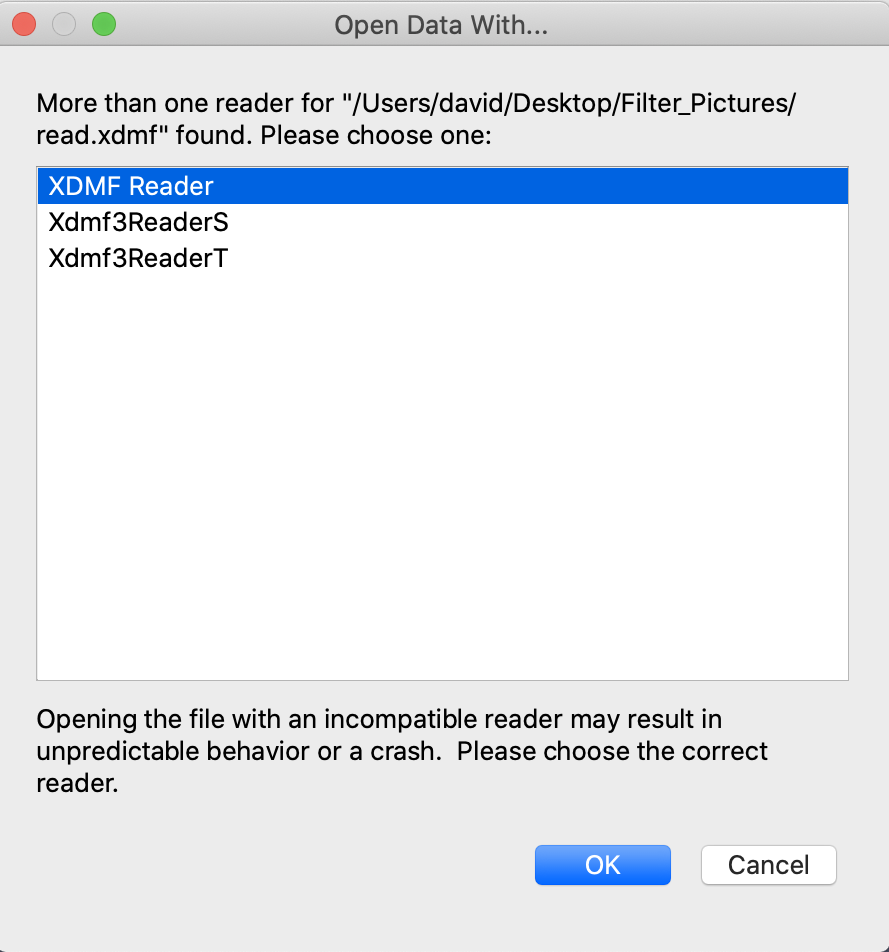
\includegraphics[width=0.7\textwidth]{./images/paraview.png}
  \caption{XDMF option for Paraview.}\label{fig:paraview}
  \end{centering}
\end{figure}

Once in Paraview, the file can be loaded by selecting \verb|File -> Open -> XDMF reader|, as in Figure \ref{fig:paraview}. Click Apply on the left hand side, and the geometry will be visible.


\subsection{Tecplot}
OpenSBLI output files can be read into Tecplot natively, selecting the HDF5Loader option when prompted. To remove the halo points select \verb|Data -> Extract -> Subzone|, and for each direction set the start and end values to 6, and $N-5$ respectively. Click 'Zone Style' on the left, and deselect 'Zone 1' to show the data without halos. This process can be repeated for multiple blocks in succession for multi-block cases. To choose the correct coordinates, select \verb|Plot -> Assign XY|, and select the coordinate arrays in the output file.

\end{document}